% !TeX program = xelatex
% !TeX encoding = UTF-8
% Presentazione revisionata: Credentia · Inferenza bayesiana
% Basata sul materiale originale fornito dall'autore e sul template M01_Pensare_con_i_dati.tex
% Compilazione: xelatex -interaction=nonstopmode M21_Credentia.tex (due passaggi)
% Diagrammi TikZ e figure statistiche vettoriali; sorgenti R e dati inclusi.
% 32 slide. Materiali del corso e impaginazione della serie planetaria.
\RequirePackage{fix-cm}
\documentclass[12pt,aspectratio=1610]{beamer}
\geometry{paperwidth=20cm,paperheight=12.5cm}
\usepackage[italian,provide=*]{babel}
\usepackage{fontspec,adjustbox,tabularx}
\IfFontExistsTF{NimbusSans-Regular.otf}{
\setsansfont{NimbusSans-Regular.otf}[BoldFont=NimbusSans-Bold.otf,ItalicFont=NimbusSans-Italic.otf,BoldItalicFont=NimbusSans-BoldItalic.otf]
\setmainfont{NimbusSans-Regular.otf}[BoldFont=NimbusSans-Bold.otf,ItalicFont=NimbusSans-Italic.otf,BoldItalicFont=NimbusSans-BoldItalic.otf]
}{
\setsansfont{TeX Gyre Heros}
\setmainfont{TeX Gyre Heros}
}
\IfFontExistsTF{DejaVu Sans Mono}{
\setmonofont{DejaVu Sans Mono}[Scale=.88]
}{\setmonofont{Latin Modern Mono}[Scale=.88]}
\usefonttheme{professionalfonts}
\usepackage{amsmath,amssymb,booktabs,array,graphicx,tikz,bookmark}
\usetikzlibrary{calc,positioning,arrows.meta}
\graphicspath{{Figure/}}
\definecolor{Paper}{HTML}{F8F6F1}
\definecolor{Ink}{HTML}{253344}
\definecolor{Navy}{HTML}{15283E}
\definecolor{Quantum}{HTML}{5146A5}
\definecolor{Classical}{HTML}{087C74}
\definecolor{Muted}{HTML}{657180}
\definecolor{Rule}{HTML}{D6DAD9}
\definecolor{Night}{HTML}{112236}
\definecolor{Lilac}{HTML}{ABB5FF}
\definecolor{Mint}{HTML}{72D8C8}
\setbeamercolor{background canvas}{bg=Paper}
\setbeamercolor{normal text}{fg=Ink}
\setbeamertemplate{navigation symbols}{}
\setbeamertemplate{headline}{}
\setbeamertemplate{footline}{}
\setbeamersize{text margin left=0pt,text margin right=0pt}
\hypersetup{colorlinks=true,linkcolor=Classical,urlcolor=Classical,pdfpagemode=UseOutlines,pdfstartview=Fit,
 pdftitle={Credentia · Inferenza bayesiana},pdfauthor={GeoStat Lab · materiali di Marzio De Corato},
 pdfsubject={GeoStat Lab · M21}}
\bookmarksetup{open,openlevel=0,depth=2}
\newsavebox{\BodyBox}
\newsavebox{\SideBox}
\newsavebox{\RecallBox}
\newsavebox{\TitleBox}
\newcommand{\MeasureBox}[2]{\typeout{REVIEWBOX:#1:\the\wd#2:\the\ht#2:\the\dp#2}}

% Revisione completa: diagrammi TikZ, formalismo e box R.
\usepackage[most]{tcolorbox}
\usepackage{listings}
\usetikzlibrary{fit,backgrounds,matrix,decorations.pathreplacing}
\definecolor{GeoA}{HTML}{1D7890}
\definecolor{GeoB}{HTML}{C57E42}
\definecolor{GeoC}{HTML}{7363AA}
\definecolor{GeoTint}{HTML}{F0F4F3}
\lstdefinestyle{GeoR}{language=R,basicstyle=\ttfamily\fontsize{9.2}{12.2}\selectfont,
 keywordstyle=\color{Quantum}\bfseries,commentstyle=\color{Classical},stringstyle=\color{GeoB},
 numbers=left,numberstyle=\tiny\color{Muted},numbersep=4pt,showstringspaces=false,
 columns=fullflexible,keepspaces=true,breaklines=true,xleftmargin=1.15em,
 frame=none,aboveskip=0pt,belowskip=0pt,tabsize=2}
\newsavebox{\PilotLeftBox}
\newsavebox{\PilotRightBox}
\newcommand{\PLabel}[1]{\par{\color{Classical}\bfseries\fontsize{9}{11}\selectfont\MakeUppercase{#1}}\par\vspace{1.8mm}}
\newcommand{\PBody}[1]{\par{\fontsize{11.3}{14.8}\selectfont #1\par}}
\newcommand{\PSmall}[1]{\par{\fontsize{9.8}{13.1}\selectfont #1\par}}
\newcommand{\PCode}[2]{%
\begin{tcolorbox}[enhanced,arc=1.8mm,boxrule=.65pt,
  colback=white,colframe=Classical!75!Navy,colbacktitle=Navy,
  coltitle=white,fonttitle=\bfseries\fontsize{9.6}{12}\selectfont,
  title={#1},left=1.7mm,right=1.3mm,top=1.5mm,bottom=1.3mm,
  before skip=1mm,after skip=1mm]
\lstinputlisting[style=GeoR]{Codice/#2}
\end{tcolorbox}}
\newcommand{\PInfo}[1]{%
\begin{tcolorbox}[enhanced,arc=1.6mm,boxrule=.55pt,colback=GeoTint,
 colframe=Rule!80!Classical,left=2.3mm,right=2.3mm,top=2mm,bottom=2mm,
 before skip=1mm,after skip=1mm]
\PSmall{#1}\end{tcolorbox}}
\tikzset{
 pFlow/.style={draw=Classical!45,fill=white,rounded corners=2mm,
  line width=.7pt,align=center,minimum height=1.1cm,font=\sffamily\fontsize{10}{12}\selectfont},
 pEdge/.style={-{Latex[length=2.3mm]},draw=Classical,line width=.95pt},
 pGroup/.style={draw=Rule,fill=white,rounded corners=2mm,line width=.65pt},
 pDotA/.style={circle,fill=GeoA,inner sep=1.25pt},
 pDotB/.style={circle,fill=GeoB,inner sep=1.25pt},
 pDotC/.style={circle,fill=GeoC,inner sep=1.25pt}
}
\newcommand{\PilotChrome}[4]{%
  \node[anchor=north west,inner sep=0,text width=17.7cm] at ([xshift=.95cm,yshift=-.55cm]current page.north west) {\color{Navy}\bfseries\fontsize{20.6}{24.5}\selectfont #1};
  \node[anchor=north east,inner sep=0] at ([xshift=19.05cm,yshift=-.14cm]current page.north west) {\color{Classical}\fontsize{8}{10}\selectfont\hyperlink{slide2}{#2}};
  \draw[Classical,line width=1.2pt] ([xshift=.95cm,yshift=-1.7cm]current page.north west)--([xshift=2.35cm,yshift=-1.7cm]current page.north west);
  \draw[Rule,line width=.65pt] ([xshift=.95cm,yshift=-10.36cm]current page.north west)--([xshift=19.05cm,yshift=-10.36cm]current page.north west);
  \node[anchor=north west,inner sep=0] at ([xshift=.96cm,yshift=-10.55cm]current page.north west) {\color{Classical}\bfseries\fontsize{9.1}{12}\selectfont DA RICORDARE};
  \node[anchor=north west,inner sep=0,text width=14.3cm] at ([xshift=4.2cm,yshift=-10.53cm]current page.north west) {\color{Ink}\fontsize{10.3}{13.8}\selectfont #4};
  \draw[Rule,line width=.35pt] ([xshift=.95cm,yshift=-11.92cm]current page.north west)--([xshift=19.05cm,yshift=-11.92cm]current page.north west);
  \node[anchor=north west,inner sep=0] at ([xshift=.95cm,yshift=-12.06cm]current page.north west) {\color{Muted}\fontsize{7.7}{9.2}\selectfont Credentia · Inferenza bayesiana};
  \node[anchor=north east,inner sep=0] at ([xshift=19.05cm,yshift=-12.06cm]current page.north west) {\color{Muted}\fontsize{7.7}{9.2}\selectfont #3/32};
}


% Stili comuni per i diagrammi scientifici della revisione completa.
\tikzset{
 pAxis/.style={-{Latex[length=2mm]},draw=Muted,line width=.65pt},
 pNote/.style={font=\sffamily\fontsize{9}{11.5}\selectfont,text=Muted,align=center},
 pLabel/.style={font=\sffamily\fontsize{10}{12.5}\selectfont,text=Ink,align=center}
}
\newsavebox{\FullWideBox}
\setlength{\emergencystretch}{1em}




\newcommand{\PLab}[2]{\par{\color{Classical}\bfseries\fontsize{9}{11}\selectfont
\href{#1}{\MakeUppercase{#2}}}\par\vspace{1.8mm}}

\definecolor{Measure}{HTML}{A05B10}\definecolor{Rose}{HTML}{9B4564}\definecolor{Wash}{HTML}{EAE7F6}\definecolor{Gold}{HTML}{EEC184}
\tikzset{arr/.style={-{Stealth[length=2mm]},line width=.8pt,draw=Classical}}
\newcommand{\Colonna}[2]{\begin{adjustbox}{max totalsize={#1}{7.95cm},valign=t}\begin{minipage}[t]{#1}\raggedright\fontsize{11.3}{14.8}\selectfont #2\end{minipage}\end{adjustbox}}
\begin{document}

\begin{frame}[plain]\hypertarget{slide1}{}\bookmark[level=0,page=1]{Credentia}
\begin{tikzpicture}[remember picture,overlay]
\fill[Night](current page.south west) rectangle(current page.north east);
\IfFileExists{Scena/copertina.jpg}{\node[inner sep=0] at(current page.center){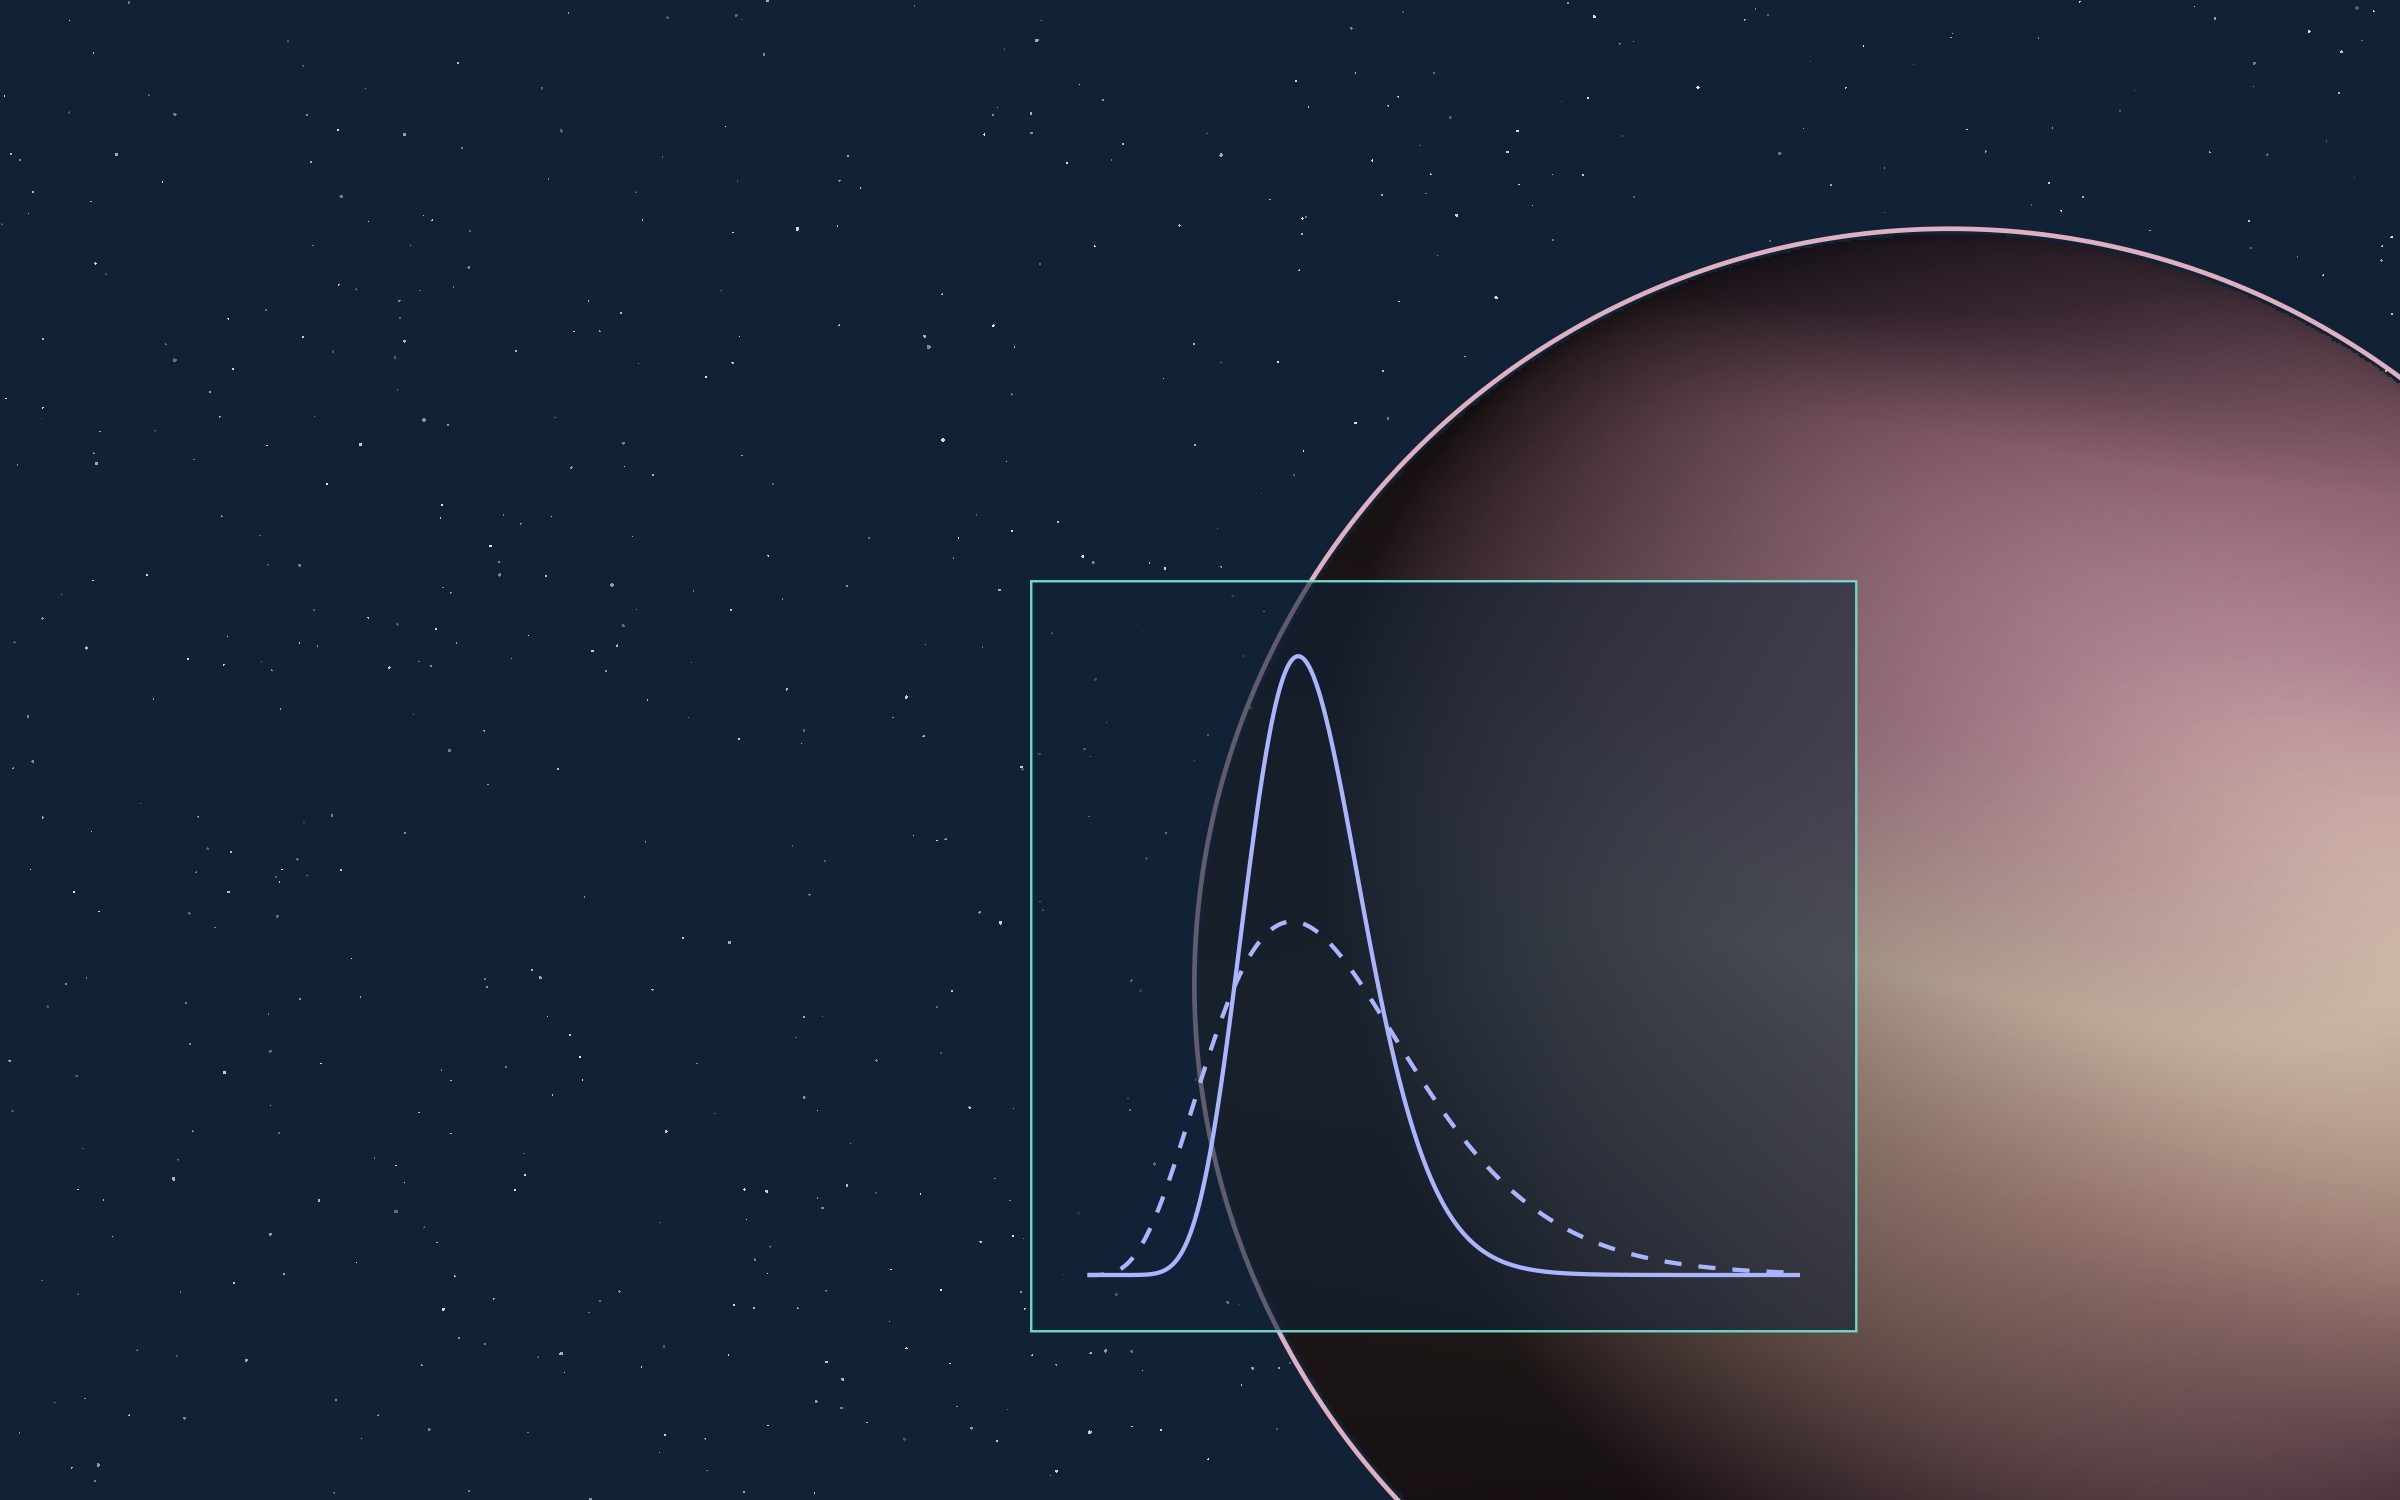
\includegraphics[width=20cm,height=12.5cm]{Scena/copertina.jpg}};}{}
\node[anchor=north west,inner sep=0] at([xshift=1.05cm,yshift=-1.10cm]current page.north west){\color{Mint}\bfseries\fontsize{23}{28}\selectfont CREDENTIA};
\node[anchor=north west,inner sep=0] at([xshift=1.07cm,yshift=-2.16cm]current page.north west){\color{white}\fontsize{9}{12}\selectfont MODULO M21 · SCIENZE DELLA TERRA};
\draw[Mint,line width=1.5pt]([xshift=1.07cm,yshift=-2.78cm]current page.north west)--([xshift=2.6cm,yshift=-2.78cm]current page.north west);
\node[anchor=north west,inner sep=0] at([xshift=1.05cm,yshift=-3.35cm]current page.north west){\begin{minipage}{9.2cm}\raggedright\color{white}\bfseries\fontsize{28.5}{34.5}\selectfont Inferenza\\bayesiana\end{minipage}};
\node[anchor=north west,inner sep=0] at([xshift=1.07cm,yshift=-7.88cm]current page.north west){\begin{minipage}{8.9cm}\raggedright\color{Lilac}\fontsize{12.2}{17}\selectfont Stimare con la distribuzione a posteriori\end{minipage}};
\node[anchor=north west,inner sep=0] at([xshift=1.07cm,yshift=-8.70cm]current page.north west){\begin{minipage}{8.9cm}\raggedright\color{white!75}\fontsize{10.3}{14.5}\selectfont Griglie, distribuzioni coniugate, scelta della distribuzione a priori e algoritmo di Metropolis\end{minipage}};
\node[anchor=north west,inner sep=0] at([xshift=1.07cm,yshift=-10.52cm]current page.north west){\color{white}\fontsize{10.5}{14}\selectfont GeoStat Lab · corso di Marzio De Corato};
\node[anchor=north west,inner sep=0] at([xshift=1.07cm,yshift=-11.17cm]current page.north west){\color{Mint}\fontsize{8.8}{11}\selectfont\href{https://creativecommons.org/licenses/by-nc-sa/4.0/}{Impaginazione da Tessera · CC BY-NC-SA 4.0}};
\end{tikzpicture}\end{frame}

\begin{frame}[plain]\hypertarget{slide2}{}
\bookmark[level=1,page=2]{Indice della presentazione}
\begin{tikzpicture}[remember picture,overlay]
\PilotChrome{Indice della presentazione}{PERCORSO}{2}{I titoli dell’indice aprono i capitoli. Il nome del capitolo in alto riporta a questa pagina.}
\node[anchor=north west,inner sep=0] at([xshift=.96cm,yshift=-2.12cm]current page.north west){\Colonna{9.40cm}{\PLabel{Capitoli}
{\fontsize{10.7}{13.5}\selectfont\hyperlink{slide4}{Il teorema di Bayes\hfill 4}\par}\vspace{.16cm}
{\fontsize{10.7}{13.5}\selectfont\hyperlink{slide10}{Coniugate e intervalli di credibilità\hfill 10}\par}\vspace{.16cm}
{\fontsize{10.7}{13.5}\selectfont\hyperlink{slide17}{Sensibilità alla distribuzione a priori\hfill 17}\par}\vspace{.16cm}
{\fontsize{10.7}{13.5}\selectfont\hyperlink{slide24}{Monte Carlo a catena di Markov\hfill 24}\par}\vspace{.16cm}
}};
\node[anchor=north west,inner sep=0] at([xshift=10.85cm,yshift=-2.12cm]current page.north west){\Colonna{8.16cm}{\PLabel{Percorso di lettura}
\PBody{Il registro storico di un vulcano conta nove eruzioni in 375 anni; quattordici vulcani analoghi forniscono un’informazione preliminare sul tasso eruttivo e sulla frazione di eruzioni esplosive. Il percorso va dal teorema di Bayes su una griglia alle distribuzioni coniugate, alla scelta della distribuzione a priori e all’algoritmo di Metropolis per i tempi di riposo.}
\PInfo{Le pagine Scenario A e Confronto riprendono gli esperimenti nel browser. I valori di partenza del simulatore possono differire dal caso guida.}
\href{https://marzione00.github.io/Lab_Geo/\#modulo-M21}{\color{Classical}\bfseries Apri gli esperimenti di Credentia}}};
\end{tikzpicture}\end{frame}

\begin{frame}[plain]\hypertarget{slide3}{}
\bookmark[level=1,page=3]{Quanto è probabile un’eruzione nei prossimi cinquant’anni?}
\begin{tikzpicture}[remember picture,overlay]
\PilotChrome{{\fontsize{15.3}{19}\selectfont Quanto è probabile un’eruzione nei prossimi cinquant’anni?}}{IL CASO GUIDA}{3}{Una distribuzione a posteriori descrive l’incertezza sul parametro dopo aver visto i dati.}
\node[anchor=north west,inner sep=0] at([xshift=.96cm,yshift=-2.12cm]current page.north west){\Colonna{9.40cm}{{\centering\resizebox{.97\linewidth}{!}{\begin{tikzpicture}[x=1cm,y=1cm,every node/.append style={anchor=center,inner sep=.3333em}]
\foreach \x/\n/\t/\col in {0.9/1/{Teorema\\di Bayes}/GeoA,3.0/2/{Coniugate}/GeoC,5.1/3/{Distribuz.\\a priori}/GeoA,7.2/4/{Catene\\di Markov}/GeoB}{
 \draw[\col,fill=\col!8,rounded corners=4pt,line width=.8pt] (\x-.95,1.25) rectangle(\x+.95,3.35);
 \node[font=\bfseries\fontsize{15}{18}\selectfont,text=\col] at(\x,2.75){\n};
 \node[pNote,text width=1.75cm,align=center] at(\x,1.85){\t};}
\foreach \x in {1.85,3.95,6.05}{\draw[pEdge] (\x,2.3)--(\x+.2,2.3);}
\draw[Rule,line width=.6pt] (0,.75)--(8.15,.75);
\node[pNote] at(4.08,.35){Un tasso, una frazione e due parametri: dalla griglia alla simulazione.};
\end{tikzpicture}
}\par}
}};
\node[anchor=north west,inner sep=0] at([xshift=10.85cm,yshift=-2.12cm]current page.north west){\Colonna{8.16cm}{\PLabel{Il caso}
\PBody{Un vulcano sintetico ha eruttato nove volte fra il 1650 e il 2025, l’ultima nel 1988; quattro eruzioni sono state esplosive. Quattordici vulcani analoghi, osservati per 140–440 anni, hanno da tre a sedici eruzioni ciascuno. Con un registro così breve l’informazione dei vulcani analoghi pesa sulla stima.}
\PInfo{Seguiremo i dati dalla griglia al teorema di Bayes in forma chiusa, alla probabilità di un’eruzione esplosiva e a un modello dei tempi di riposo stimato con una catena di Markov.}
}};
\end{tikzpicture}\end{frame}

\begin{frame}[plain]\hypertarget{slide4}{}
\bookmark[level=0,page=4]{Il teorema di Bayes}
\bookmark[level=1,page=4]{Che cosa dice il solo registro?}
\begin{tikzpicture}[remember picture,overlay]
\PilotChrome{Che cosa dice il solo registro?}{IL TEOREMA DI BAYES}{4}{Sostituire il tasso stimato nella formula della probabilità ignora l’incertezza della stima.}
\node[anchor=north west,inner sep=0] at([xshift=.96cm,yshift=-2.12cm]current page.north west){\Colonna{9.40cm}{\PLabel{Domanda}
\PBody{Nove eruzioni in 3,75 secoli danno un tasso di 2,4 eruzioni per secolo. Quanto è incerto? Che probabilità di almeno un’eruzione in mezzo secolo si ottiene inserendo il tasso stimato nella formula di Poisson?}
\vspace{.35cm}\PLabel{Interpretazione}
\PBody{L’intervallo esatto di Garwood al 95\% va da 1,10 a 4,56 eruzioni per secolo: un fattore quattro. La formula $1-e^{-0{,}5\lambda}$ con $\lambda=2{,}4$ dà 0,699, un numero che non porta traccia di questa incertezza.}
}};
\node[anchor=north west,inner sep=0] at([xshift=10.85cm,yshift=-2.12cm]current page.north west){\Colonna{8.16cm}{\begin{tcolorbox}[enhanced,arc=1.7mm,boxrule=.6pt,colback=white,colframe=Classical!60!Navy,colbacktitle=Navy,coltitle=white,fonttitle=\bfseries\small,title={R · calcolo riproducibile},left=1.7mm,right=1.3mm,top=1.1mm,bottom=1.1mm,before skip=1mm,after skip=1.0mm]\lstinputlisting[style=GeoR,language=R]{Codice/capitolo-01.R}\end{tcolorbox}
\PLabel{Risultato in R}
\begin{tcolorbox}[colback=GeoTint,colframe=Rule,boxrule=.5pt,arc=1.4mm,left=2mm,right=1mm,top=1mm,bottom=1mm]{\fontsize{8.6}{11.4}\selectfont\ttfamily \mbox{eruzioni\ \ \ secoli\ \ \ \ stima}\\\mbox{\ \ \ \ 9.00\ \ \ \ \ 3.75\ \ \ \ \ 2.40}\\\mbox{[1]\ 1.097433\ 4.555948}\\\mbox{[1]\ 0.6988058}}\end{tcolorbox}}};
\end{tikzpicture}\end{frame}

\begin{frame}[plain]\hypertarget{slide5}{}
\bookmark[level=1,page=5]{Distribuzione a priori, verosimiglianza e distribuzione a posteriori}
\begin{tikzpicture}[remember picture,overlay]
\PilotChrome{{\fontsize{15.3}{19}\selectfont Distribuzione a priori, verosimiglianza e distribuzione a posteriori}}{IL TEOREMA DI BAYES}{5}{La distribuzione a posteriori è proporzionale al prodotto di distribuzione a priori e verosimiglianza.}
\node[anchor=north west,inner sep=0] at([xshift=.96cm,yshift=-2.12cm]current page.north west){\Colonna{9.40cm}{{\centering\resizebox{0.94\linewidth}{!}{\begin{tikzpicture}[x=1cm,y=1cm,every node/.append style={anchor=center,inner sep=.3333em}]
\node[pFlow,text width=2.5cm] (a) at(0,2.5){\textbf{A priori}\\$\pi(\lambda)$\\vulcani analoghi};
\node[pFlow,text width=2.9cm] (b) at(5.8,2.5){\textbf{Verosimiglianza}\\$p(N\mid\lambda)$\\registro storico};
\node[pFlow,text width=3.1cm] (c) at(2.9,0){\textbf{A posteriori}\\$\pi(\lambda\mid N)\propto p(N\mid\lambda)\,\pi(\lambda)$};
\draw[pEdge] (a)--(c);
\draw[pEdge] (b)--(c);
\node[pNote,text width=7.4cm] at(2.9,-1.7){La costante di normalizzazione $p(N)=\int p(N\mid\lambda)\pi(\lambda)\,d\lambda$ rende l’area uguale a 1: su una griglia è una somma.};
\end{tikzpicture}
}\par}
\PSmall{Il teorema di Bayes applicato al tasso eruttivo.}
}};
\node[anchor=north west,inner sep=0] at([xshift=10.85cm,yshift=-2.12cm]current page.north west){\Colonna{8.16cm}{\PBody{Thomas Bayes affrontò il problema di risalire da un numero di successi alla probabilità che li ha prodotti; il saggio fu pubblicato nel 1763, dopo la sua morte. In forma moderna il parametro ha una distribuzione di probabilità: quella a priori riassume l’informazione disponibile prima dei dati, e i dati la aggiornano attraverso la verosimiglianza.}
\par\smallskip{\centering\adjustbox{max width=.98\linewidth}{$\displaystyle \pi(\lambda\mid N)=\frac{p(N\mid\lambda)\,\pi(\lambda)}{p(N)}$}\par\smallskip}
}};
\end{tikzpicture}\end{frame}

\begin{frame}[plain]\hypertarget{slide6}{}
\bookmark[level=1,page=6]{La distribuzione a posteriori su una griglia}
\begin{tikzpicture}[remember picture,overlay]
\PilotChrome{La distribuzione a posteriori su una griglia}{IL TEOREMA DI BAYES}{6}{Su una griglia il teorema di Bayes è un prodotto seguito da una normalizzazione.}
\node[anchor=north west,inner sep=0] at([xshift=.96cm,yshift=-2.12cm]current page.north west){\Colonna{9.40cm}{\PBody{Il codice valuta distribuzione a priori uniforme e verosimiglianza di Poisson in 4001 punti fra 0 e 10 eruzioni per secolo, divide il prodotto per la sua area e ricava media e quantili. La media a posteriori vale 2,67 e l’intervallo di credibilità al 95\% va da 1,28 a 4,56: c’è una probabilità di 0,95 che il tasso stia in questo intervallo.}
\par\smallskip{\centering\adjustbox{max width=.98\linewidth}{$\displaystyle \pi(\lambda_j\mid N)\approx\frac{p(N\mid\lambda_j)\,\pi(\lambda_j)}{\sum_i p(N\mid\lambda_i)\,\pi(\lambda_i)\,\Delta}$}\par\smallskip}
}};
\node[anchor=north west,inner sep=0] at([xshift=10.85cm,yshift=-2.12cm]current page.north west){\Colonna{8.16cm}{\begin{tcolorbox}[enhanced,arc=1.7mm,boxrule=.6pt,colback=white,colframe=Classical!60!Navy,colbacktitle=Navy,coltitle=white,fonttitle=\bfseries\small,title={R · calcolo riproducibile},left=1.7mm,right=1.3mm,top=1.1mm,bottom=1.1mm,before skip=1mm,after skip=1.0mm]\lstinputlisting[style=GeoR,language=R]{Codice/capitolo-02.R}\end{tcolorbox}
\PLabel{Risultato in R}
\begin{tcolorbox}[colback=GeoTint,colframe=Rule,boxrule=.5pt,arc=1.4mm,left=2mm,right=1mm,top=1mm,bottom=1mm]{\fontsize{8.6}{11.4}\selectfont\ttfamily \mbox{\ \ \ media\ \ \ \ \ \ inf\ \ \ \ \ \ sup}\\\mbox{2.666666\ 1.280000\ 4.555000}}\end{tcolorbox}}};
\end{tikzpicture}\end{frame}

\begin{frame}[plain]\hypertarget{slide7}{}
\bookmark[level=1,page=7]{Prima e dopo il registro storico}
\begin{tikzpicture}[remember picture,overlay]
\PilotChrome{Prima e dopo il registro storico}{IL TEOREMA DI BAYES}{7}{La distribuzione a posteriori sta fra la distribuzione a priori e la verosimiglianza, ed è più stretta di entrambe.}
\node[anchor=north west,inner sep=0] at([xshift=.96cm,yshift=-2.12cm]current page.north west){\Colonna{9.40cm}{{\centering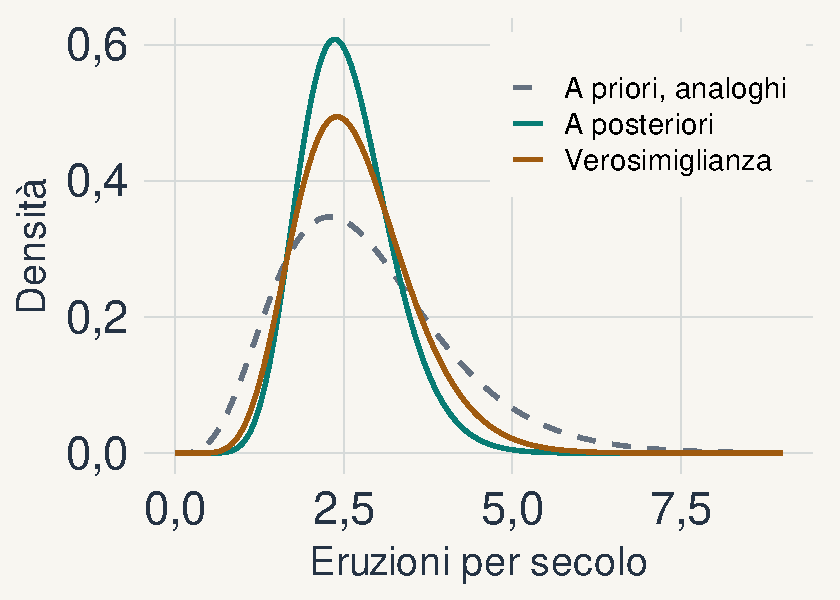
\includegraphics[width=\linewidth,height=6.15cm,keepaspectratio]{Figure/F01.pdf}\par}
\PSmall{Densità a priori dai vulcani analoghi, verosimiglianza normalizzata e densità a posteriori del tasso eruttivo.}
}};
\node[anchor=north west,inner sep=0] at([xshift=10.85cm,yshift=-2.12cm]current page.north west){\Colonna{8.16cm}{\PBody{La distribuzione a priori dei vulcani analoghi ha media 2,85 eruzioni per secolo ed è larga, da 0,94 a 5,78. La verosimiglianza del registro è centrata su 2,4. La distribuzione a posteriori ha media 2,55 e intervallo da 1,40 a 4,03, più stretto di entrambe: combina due fonti di informazione.}
\PSmall{La verosimiglianza normalizzata coincide con la distribuzione a posteriori ottenuta da una distribuzione a priori uniforme.}
}};
\end{tikzpicture}\end{frame}

\begin{frame}[plain]\hypertarget{slide8}{}
\bookmark[level=1,page=8]{Distribuzione a posteriori e lunghezza del registro}
\begin{tikzpicture}[remember picture,overlay]
\PilotChrome{Distribuzione a posteriori e lunghezza del registro}{IL TEOREMA DI BAYES}{8}{Valutare quanto la distribuzione a posteriori dipende dalla distribuzione a priori al variare della quantità di dati.}
\node[anchor=north west,inner sep=0] at([xshift=.96cm,yshift=-2.12cm]current page.north west){\Colonna{9.40cm}{{\centering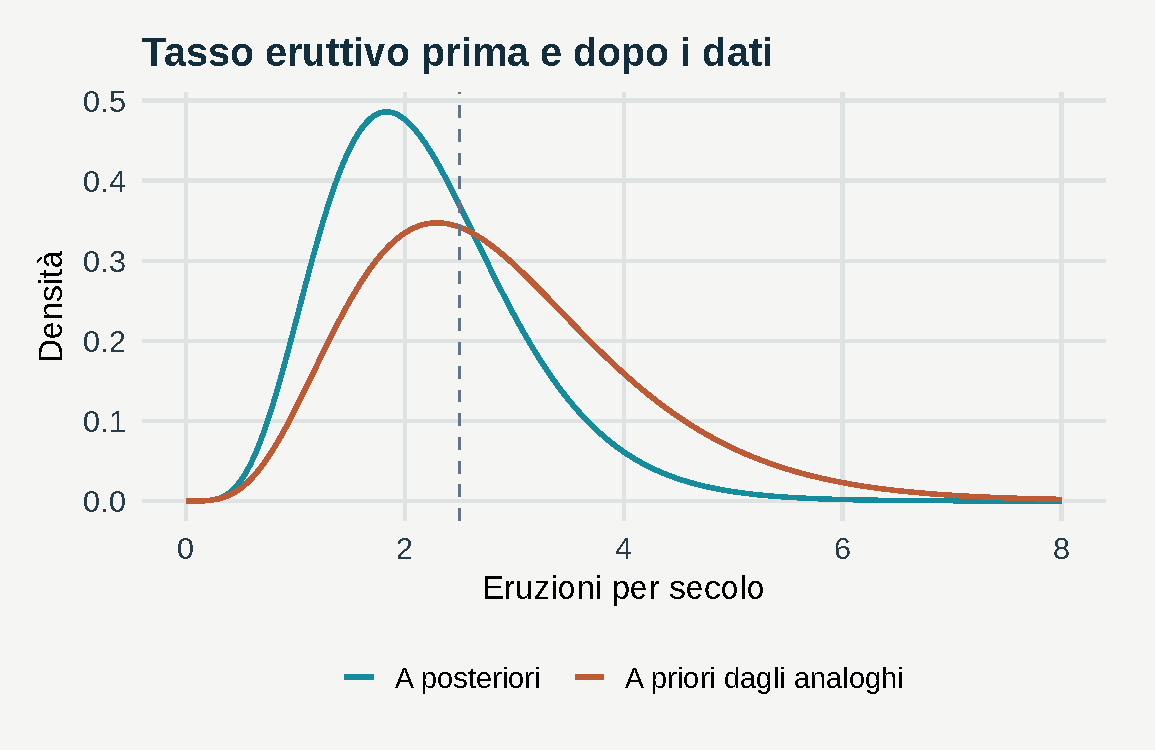
\includegraphics[width=\linewidth,height=6.0cm,keepaspectratio]{Esperimenti/m21-registro-A.pdf}\par}
\PSmall{Registro di un secolo; tasso vero 2,5 eruzioni per secolo. Seme: 17.}
}};
\node[anchor=north west,inner sep=0] at([xshift=10.85cm,yshift=-2.12cm]current page.north west){\Colonna{8.16cm}{\PLabel{Scenario A · simulazione}
\PBody{L’esperimento genera il numero di eruzioni di un registro della durata scelta e aggiorna la distribuzione a priori dei vulcani analoghi. Con un secolo di registro si osserva un’eruzione: la media a posteriori vale 2,19 e l’intervallo al 95\% è ampio 3,41 eruzioni per secolo.}
\par\smallskip{\centering\adjustbox{max width=.98\linewidth}{$\displaystyle \lambda\mid N\sim\mathrm{Gamma}(a+N,\;b+T)$}\par\smallskip}
\PSmall{Il peso della distribuzione a priori nella media a posteriori vale $b/(b+T)=0{,}644$.}
}};
\node[anchor=north east,inner sep=0] at([xshift=17.1cm,yshift=-12.04cm]current page.north west){\fontsize{7.7}{9}\selectfont \href{https://marzione00.github.io/Lab_Geo/\#laboratorio/m21-registro}{\color{Classical}\bfseries Apri il laboratorio · m21-registro}};
\end{tikzpicture}\end{frame}

\begin{frame}[plain]\hypertarget{slide9}{}
\bookmark[level=1,page=9]{Confronto | Lunghezza del registro}
\begin{tikzpicture}[remember picture,overlay]
\PilotChrome{Confronto | Lunghezza del registro}{IL TEOREMA DI BAYES}{9}{Con più dati la distribuzione a priori conta meno e l’intervallo si restringe.}
\node[anchor=north west,inner sep=0] at([xshift=.96cm,yshift=-2.12cm]current page.north west){\Colonna{9.40cm}{{\centering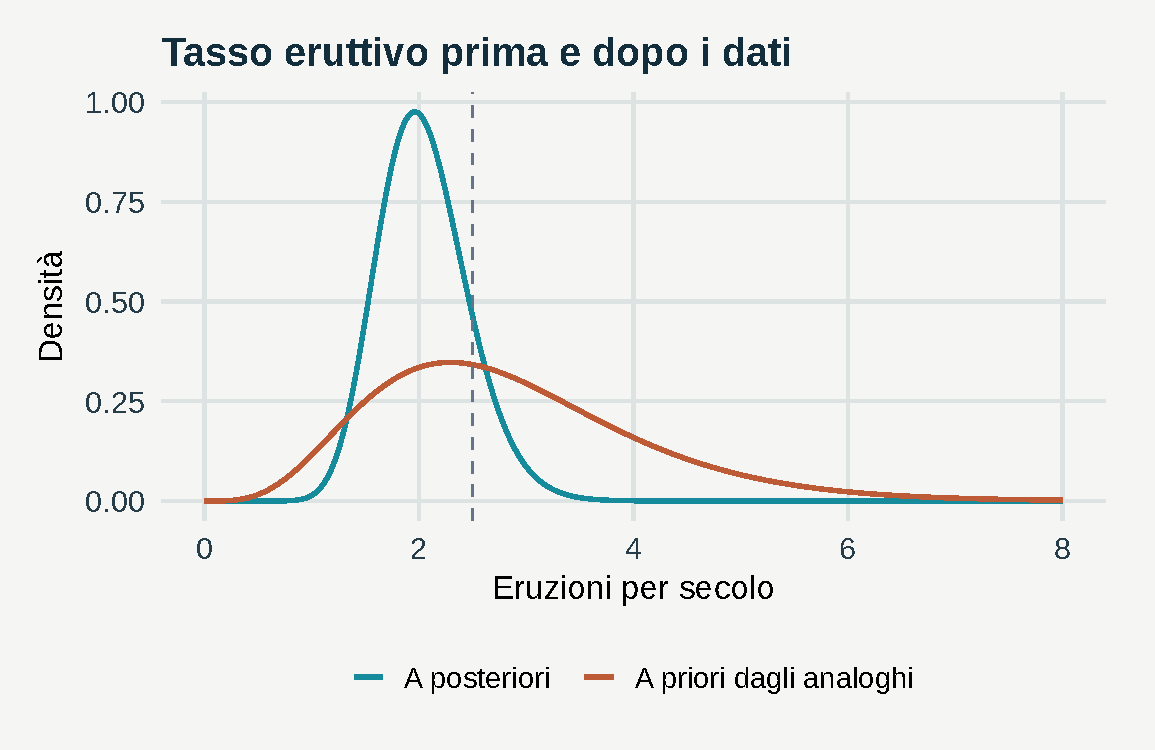
\includegraphics[width=\linewidth,height=5.6cm,keepaspectratio]{Esperimenti/m21-registro-B.pdf}\par}
\PSmall{Durata del registro: 1 $\to$ 10 secoli. Il seme è fisso.}
}};
\node[anchor=north west,inner sep=0] at([xshift=10.85cm,yshift=-2.12cm]current page.north west){\Colonna{8.16cm}{\PLabel{Confronto fra gli scenari}
{\fontsize{10.2}{12.8}\selectfont\begin{tabular}{@{}>{\raggedright\arraybackslash}p{0.48\linewidth}@{\hspace{.13cm}}>{\raggedright\arraybackslash}p{0.224\linewidth}@{\hspace{.13cm}}>{\raggedright\arraybackslash}p{0.224\linewidth}@{}}\toprule Grandezza & A & B\\[2.3pt]
\midrule 
Eruzioni osservate & 1 & 19\\[2.3pt]
Media a posteriori & 2{,}19 & 2{,}04\\[2.3pt]
Ampiezza dell’intervallo & 3{,}41 & 1{,}63\\[2.3pt]
Peso della distribuzione a priori & 0{,}644 & 0{,}153\\[2.3pt]
\bottomrule\end{tabular}\par}
\vspace{.25cm}\PBody{Con dieci secoli si osservano 19 eruzioni contro 25 attese, e la media a posteriori vale 2,04. Il peso della distribuzione a priori scende a 0,153 e l’intervallo si restringe a 1,63.}
}};
\node[anchor=north east,inner sep=0] at([xshift=17.1cm,yshift=-12.04cm]current page.north west){\fontsize{7.7}{9}\selectfont \href{https://marzione00.github.io/Lab_Geo/\#laboratorio/m21-registro}{\color{Classical}\bfseries Apri il laboratorio · m21-registro}};
\end{tikzpicture}\end{frame}

\begin{frame}[plain]\hypertarget{slide10}{}
\bookmark[level=0,page=10]{Coniugate e intervalli di credibilità}
\bookmark[level=1,page=10]{Un aggiornamento in forma chiusa}
\begin{tikzpicture}[remember picture,overlay]
\PilotChrome{Un aggiornamento in forma chiusa}{CONIUGATE E INTERVALLI DI CREDIBILITÀ}{10}{Con una distribuzione a priori coniugata la distribuzione a posteriori appartiene alla stessa famiglia.}
\node[anchor=north west,inner sep=0] at([xshift=.96cm,yshift=-2.12cm]current page.north west){\Colonna{9.40cm}{{\centering\resizebox{0.94\linewidth}{!}{\begin{tikzpicture}[x=1cm,y=1cm,every node/.append style={anchor=center,inner sep=.3333em}]
\node[pFlow,text width=2.6cm] (a) at(0,2.4){\textbf{A priori}\\$\mathrm{Gamma}(a,b)$\\$a$ eruzioni in $b$ secoli};
\node[pFlow,text width=2.6cm] (b) at(5.8,2.4){\textbf{Dati}\\$N$ eruzioni\\in $T$ secoli};
\node[pFlow,text width=3.9cm] (c) at(2.9,0){\textbf{A posteriori}\\$\mathrm{Gamma}(a+N,\;b+T)$};
\draw[pEdge] (a)--(c);
\draw[pEdge] (b)--(c);
\node[pNote,text width=7.6cm] at(2.9,-1.6){Media a posteriori $\dfrac{a+N}{b+T}=w\,\dfrac{a}{b}+(1-w)\,\dfrac{N}{T}$, con peso $w=\dfrac{b}{b+T}$ per la distribuzione a priori.};
\end{tikzpicture}
}\par}
\PSmall{Aggiornamento della gamma con un registro di Poisson.}
}};
\node[anchor=north west,inner sep=0] at([xshift=10.85cm,yshift=-2.12cm]current page.north west){\Colonna{8.16cm}{\PBody{Se la distribuzione a priori del tasso è una gamma e le eruzioni seguono un processo di Poisson, anche la distribuzione a posteriori è una gamma: la forma aumenta del numero di eruzioni, il parametro di scala inverso della durata. I due parametri della distribuzione a priori si leggono come un registro immaginario di $a$ eruzioni in $b$ secoli.}
\par\smallskip{\centering\adjustbox{max width=.98\linewidth}{$\displaystyle \mathrm{Gamma}(a,b)\to\mathrm{Gamma}(a+N,b+T)$}\par\smallskip}
}};
\end{tikzpicture}\end{frame}

\begin{frame}[plain]\hypertarget{slide11}{}
\bookmark[level=1,page=11]{La distribuzione a priori dei vulcani analoghi}
\begin{tikzpicture}[remember picture,overlay]
\PilotChrome{La distribuzione a priori dei vulcani analoghi}{CONIUGATE E INTERVALLI DI CREDIBILITÀ}{11}{Se i tassi seguono una gamma, i conteggi dei vulcani analoghi seguono una binomiale negativa.}
\node[anchor=north west,inner sep=0] at([xshift=.96cm,yshift=-2.12cm]current page.north west){\Colonna{9.40cm}{\PBody{Il codice stima i parametri della gamma massimizzando la verosimiglianza binomiale negativa dei conteggi dei quattordici vulcani analoghi: $a=5{,}15$ e $b=1{,}81$ secoli. Aggiunge poi le nove eruzioni del caso: la distribuzione a posteriori è una gamma con parametri 14,15 e 5,56, media 2,55 e intervallo da 1,40 a 4,03.}
\par\smallskip{\centering\adjustbox{max width=.98\linewidth}{$\displaystyle N_j\sim\mathrm{BN}\Big(a,\;\mu_j=\frac{a}{b}\,T_j\Big)$}\par\smallskip}
}};
\node[anchor=north west,inner sep=0] at([xshift=10.85cm,yshift=-2.12cm]current page.north west){\Colonna{8.16cm}{\begin{tcolorbox}[enhanced,arc=1.7mm,boxrule=.6pt,colback=white,colframe=Classical!60!Navy,colbacktitle=Navy,coltitle=white,fonttitle=\bfseries\small,title={R · calcolo riproducibile},left=1.7mm,right=1.3mm,top=1.1mm,bottom=1.1mm,before skip=1mm,after skip=1.0mm]\lstinputlisting[style=GeoR,language=R]{Codice/capitolo-03.R}\end{tcolorbox}
\PLabel{Risultato in R}
\begin{tcolorbox}[colback=GeoTint,colframe=Rule,boxrule=.5pt,arc=1.4mm,left=2mm,right=1mm,top=1mm,bottom=1mm]{\fontsize{8.6}{11.4}\selectfont\ttfamily \mbox{\ \ \ \ \ A\ \ \ \ \ \ B\ \ \ \ \ A1\ \ \ \ \ B1\ \ media}\\\mbox{\ 5.147\ \ 1.807\ 14.147\ \ 5.557\ \ 2.546}\\\mbox{[1]\ 1.397\ 4.033}}\end{tcolorbox}}};
\end{tikzpicture}\end{frame}

\begin{frame}[plain]\hypertarget{slide12}{}
\bookmark[level=1,page=12]{Quattordici vulcani analoghi}
\begin{tikzpicture}[remember picture,overlay]
\PilotChrome{Quattordici vulcani analoghi}{CONIUGATE E INTERVALLI DI CREDIBILITÀ}{12}{I vulcani analoghi differiscono fra loro più di quanto spieghino i loro registri.}
\node[anchor=north west,inner sep=0] at([xshift=.96cm,yshift=-2.12cm]current page.north west){\Colonna{9.40cm}{{\centering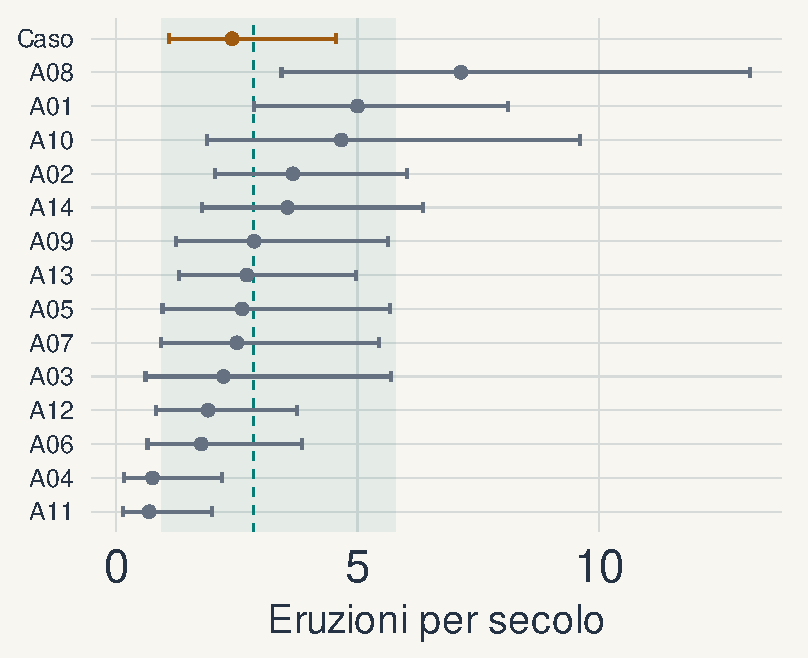
\includegraphics[width=\linewidth,height=6.15cm,keepaspectratio]{Figure/F02.pdf}\par}
\PSmall{Tassi dei vulcani analoghi e del caso con intervalli esatti al 95\%; fascia: intervallo della gamma a priori; tratteggio: sua media.}
}};
\node[anchor=north west,inner sep=0] at([xshift=10.85cm,yshift=-2.12cm]current page.north west){\Colonna{8.16cm}{\PBody{I tassi dei vulcani analoghi vanno da 0,68 a 7,14 eruzioni per secolo. La gamma stimata descrive questa variabilità fra vulcani: è la distribuzione dei tassi da cui il vulcano del caso è pensato come estratto. Il registro del caso, 2,4 eruzioni per secolo, cade vicino alla media dei vulcani analoghi.}
\PSmall{Questo uso dei dati per costruire la distribuzione a priori si chiama bayesiano empirico.}
}};
\end{tikzpicture}\end{frame}

\begin{frame}[plain]\hypertarget{slide13}{}
\bookmark[level=1,page=13]{Qual è la probabilità di un’eruzione in mezzo secolo?}
\begin{tikzpicture}[remember picture,overlay]
\PilotChrome{{\fontsize{15.3}{19}\selectfont Qual è la probabilità di un’eruzione in mezzo secolo?}}{CONIUGATE E INTERVALLI DI CREDIBILITÀ}{13}{La distribuzione predittiva media la probabilità su tutti i valori plausibili del parametro.}
\node[anchor=north west,inner sep=0] at([xshift=.96cm,yshift=-2.12cm]current page.north west){\Colonna{9.40cm}{\PLabel{Domanda}
\PBody{La distribuzione a posteriori del tasso è una gamma con parametri 14,15 e 5,56. Qual è la probabilità di almeno un’eruzione nei prossimi cinquant’anni, mediata sull’incertezza del tasso?}
\vspace{.35cm}\PLabel{Interpretazione}
\PBody{La media di $1-e^{-0{,}5\lambda}$ sulla distribuzione a posteriori ha una formula chiusa e vale 0,704; centomila estrazioni dalla gamma danno 0,705. Con il solo tasso stimato si otteneva 0,699.}
}};
\node[anchor=north west,inner sep=0] at([xshift=10.85cm,yshift=-2.12cm]current page.north west){\Colonna{8.16cm}{\begin{tcolorbox}[enhanced,arc=1.7mm,boxrule=.6pt,colback=white,colframe=Classical!60!Navy,colbacktitle=Navy,coltitle=white,fonttitle=\bfseries\small,title={R · calcolo riproducibile},left=1.7mm,right=1.3mm,top=1.1mm,bottom=1.1mm,before skip=1mm,after skip=1.0mm]\lstinputlisting[style=GeoR,language=R]{Codice/capitolo-04.R}\end{tcolorbox}
\PLabel{Risultato in R}
\begin{tcolorbox}[colback=GeoTint,colframe=Rule,boxrule=.5pt,arc=1.4mm,left=2mm,right=1mm,top=1mm,bottom=1mm]{\fontsize{8.6}{11.4}\selectfont\ttfamily \mbox{predittiva\ \ con\_stima}\\\mbox{\ 0.7044308\ \ 0.6988058}\\\mbox{[1]\ 0.7045884}}\end{tcolorbox}}};
\end{tikzpicture}\end{frame}

\begin{frame}[plain]\hypertarget{slide14}{}
\bookmark[level=1,page=14]{Quante eruzioni nei prossimi cinquant’anni}
\begin{tikzpicture}[remember picture,overlay]
\PilotChrome{Quante eruzioni nei prossimi cinquant’anni}{CONIUGATE E INTERVALLI DI CREDIBILITÀ}{14}{L’incertezza sul tasso allarga la distribuzione dei conteggi futuri.}
\node[anchor=north west,inner sep=0] at([xshift=.96cm,yshift=-2.12cm]current page.north west){\Colonna{9.40cm}{{\centering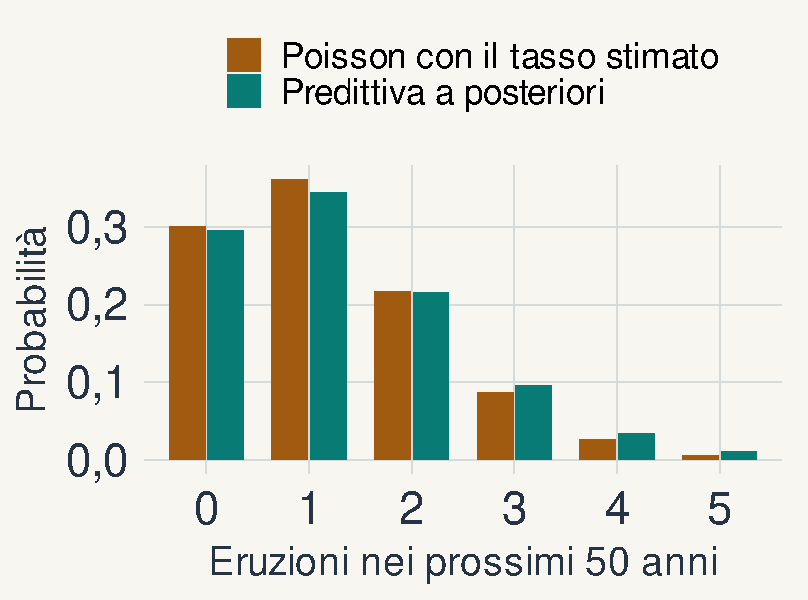
\includegraphics[width=\linewidth,height=6.15cm,keepaspectratio]{Figure/F03.pdf}\par}
\PSmall{Distribuzione predittiva a posteriori e distribuzione di Poisson con il tasso stimato.}
}};
\node[anchor=north west,inner sep=0] at([xshift=10.85cm,yshift=-2.12cm]current page.north west){\Colonna{8.16cm}{\PBody{La distribuzione predittiva a posteriori è una binomiale negativa. Rispetto alla distribuzione di Poisson con il tasso stimato assegna una probabilità minore a una o due eruzioni e maggiore a tre o più: 0,143 contro 0,121. La probabilità di nessuna eruzione cambia poco, 0,296 contro 0,301.}
\par\smallskip{\centering\adjustbox{max width=.98\linewidth}{$\displaystyle P(M=0)=\Big(\frac{b+T}{b+T+h}\Big)^{a+N}$}\par\smallskip}
}};
\end{tikzpicture}\end{frame}

\begin{frame}[plain]\hypertarget{slide15}{}
\bookmark[level=1,page=15]{Intervalli per un tasso con pochi eventi}
\begin{tikzpicture}[remember picture,overlay]
\PilotChrome{Intervalli per un tasso con pochi eventi}{CONIUGATE E INTERVALLI DI CREDIBILITÀ}{15}{Confrontare la copertura di intervalli frequentisti e di credibilità quando gli eventi sono pochi.}
\node[anchor=north west,inner sep=0] at([xshift=.96cm,yshift=-2.12cm]current page.north west){\Colonna{9.40cm}{{\centering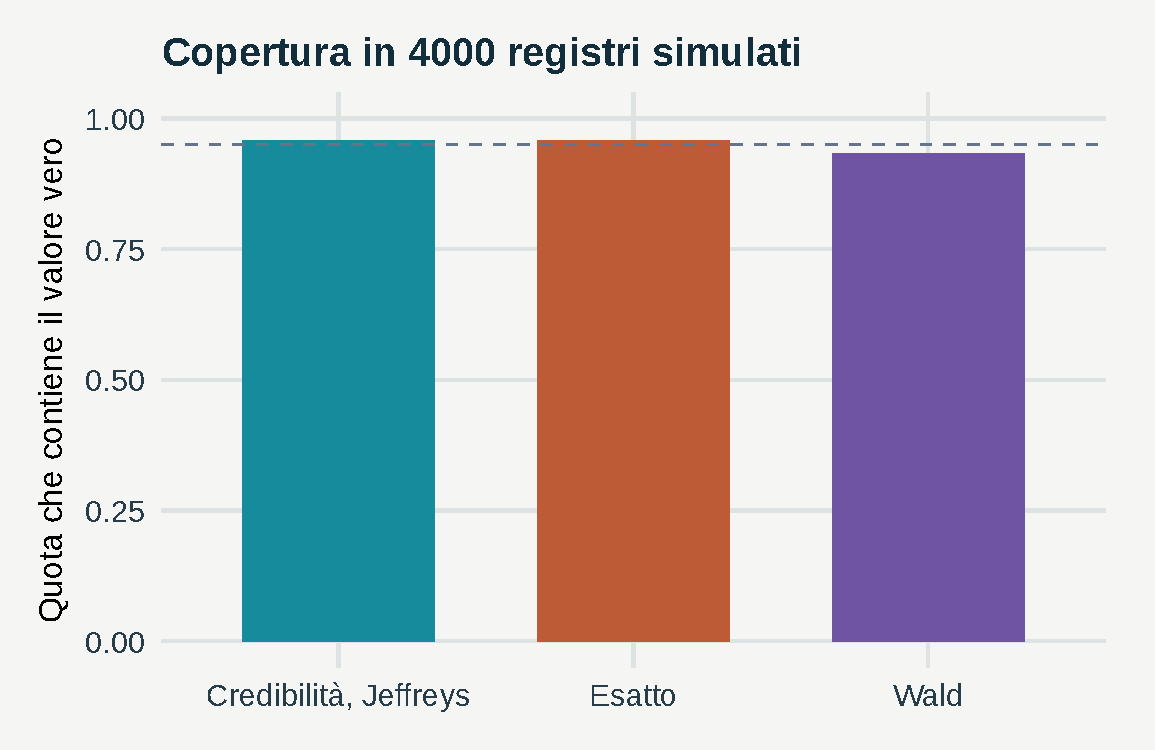
\includegraphics[width=\linewidth,height=6.0cm,keepaspectratio]{Esperimenti/m21-copertura-A.pdf}\par}
\PSmall{Trenta eventi attesi; quattromila registri. Seme: 17.}
}};
\node[anchor=north west,inner sep=0] at([xshift=10.85cm,yshift=-2.12cm]current page.north west){\Colonna{8.16cm}{\PLabel{Scenario A · simulazione}
\PBody{L’esperimento genera quattromila conteggi di Poisson e costruisce tre intervalli al 95\%: Wald, credibilità con la distribuzione a priori di Jeffreys, esatto. Con trenta eventi attesi le coperture valgono 0,933, 0,959 e 0,959.}
\par\smallskip{\centering\adjustbox{max width=.98\linewidth}{$\displaystyle \lambda\mid N\sim\mathrm{Gamma}\big(N+\tfrac12,\;1\big)$}\par\smallskip}
\PSmall{La distribuzione a priori di Jeffreys per un tasso di Poisson è proporzionale a $\lambda^{-1/2}$.}
}};
\node[anchor=north east,inner sep=0] at([xshift=17.1cm,yshift=-12.04cm]current page.north west){\fontsize{7.7}{9}\selectfont \href{https://marzione00.github.io/Lab_Geo/\#laboratorio/m21-copertura}{\color{Classical}\bfseries Apri il laboratorio · m21-copertura}};
\end{tikzpicture}\end{frame}

\begin{frame}[plain]\hypertarget{slide16}{}
\bookmark[level=1,page=16]{Confronto | Intervalli con pochi eventi}
\begin{tikzpicture}[remember picture,overlay]
\PilotChrome{Confronto | Intervalli con pochi eventi}{CONIUGATE E INTERVALLI DI CREDIBILITÀ}{16}{Con pochi eventi l’approssimazione normale fallisce; l’intervallo di Jeffreys tiene.}
\node[anchor=north west,inner sep=0] at([xshift=.96cm,yshift=-2.12cm]current page.north west){\Colonna{9.40cm}{{\centering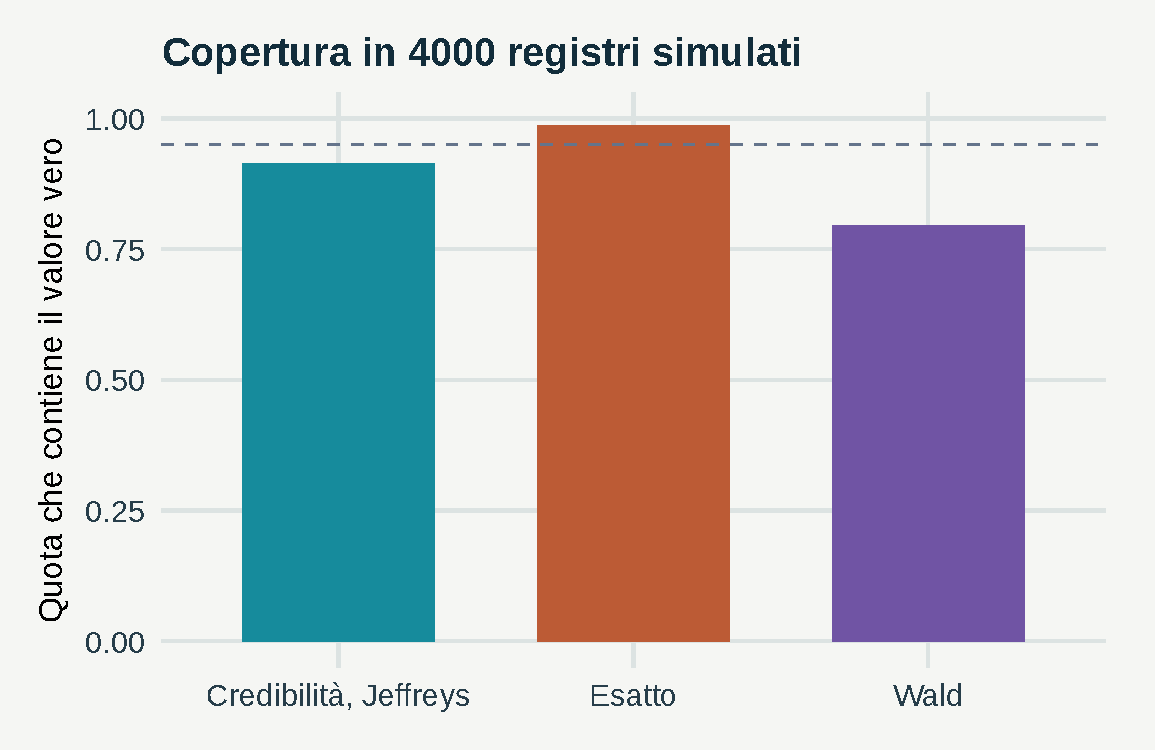
\includegraphics[width=\linewidth,height=5.6cm,keepaspectratio]{Esperimenti/m21-copertura-B.pdf}\par}
\PSmall{Eventi attesi: 30 $\to$ 3. Il seme è fisso.}
}};
\node[anchor=north west,inner sep=0] at([xshift=10.85cm,yshift=-2.12cm]current page.north west){\Colonna{8.16cm}{\PLabel{Confronto fra gli scenari}
{\fontsize{10.2}{12.8}\selectfont\begin{tabular}{@{}>{\raggedright\arraybackslash}p{0.48\linewidth}@{\hspace{.13cm}}>{\raggedright\arraybackslash}p{0.224\linewidth}@{\hspace{.13cm}}>{\raggedright\arraybackslash}p{0.224\linewidth}@{}}\toprule Grandezza & A & B\\[2.3pt]
\midrule 
Copertura, Wald & 0{,}933 & 0{,}796\\[2.3pt]
Copertura, Jeffreys & 0{,}959 & 0{,}915\\[2.3pt]
Copertura, esatto & 0{,}959 & 0{,}987\\[2.3pt]
Registri senza eventi & 0 & 0{,}0508\\[2.3pt]
\bottomrule\end{tabular}\par}
\vspace{.25cm}\PBody{Con tre eventi attesi l’intervallo di Wald contiene il valore vero nel 79,6\% dei registri, quello di Jeffreys nel 91,5\%, quello esatto nel 98,7\%. Il 5,1\% dei registri non ha eventi.}
}};
\node[anchor=north east,inner sep=0] at([xshift=17.1cm,yshift=-12.04cm]current page.north west){\fontsize{7.7}{9}\selectfont \href{https://marzione00.github.io/Lab_Geo/\#laboratorio/m21-copertura}{\color{Classical}\bfseries Apri il laboratorio · m21-copertura}};
\end{tikzpicture}\end{frame}

\begin{frame}[plain]\hypertarget{slide17}{}
\bookmark[level=0,page=17]{Sensibilità alla distribuzione a priori}
\bookmark[level=1,page=17]{La frazione di eruzioni esplosive}
\begin{tikzpicture}[remember picture,overlay]
\PilotChrome{La frazione di eruzioni esplosive}{SENSIBILITÀ ALLA DISTRIBUZIONE A PRIORI}{17}{Per una proporzione la distribuzione beta è coniugata della binomiale.}
\node[anchor=north west,inner sep=0] at([xshift=.96cm,yshift=-2.12cm]current page.north west){\Colonna{9.40cm}{\PBody{Quattro eruzioni su nove sono state esplosive. Il codice aggiorna tre distribuzioni beta a priori: uniforme, di Jeffreys e quella stimata dai vulcani analoghi, con media 0,334 e forza pari a 20 eruzioni. Le prime due danno medie a posteriori di 0,455 e 0,450 con intervalli larghi; la terza 0,368, da 0,206 a 0,548.}
\par\smallskip{\centering\adjustbox{max width=.98\linewidth}{$\displaystyle p\mid k\sim\mathrm{Beta}(\alpha+k,\;\beta+n-k)$}\par\smallskip}
}};
\node[anchor=north west,inner sep=0] at([xshift=10.85cm,yshift=-2.12cm]current page.north west){\Colonna{8.16cm}{\begin{tcolorbox}[enhanced,arc=1.7mm,boxrule=.6pt,colback=white,colframe=Classical!60!Navy,colbacktitle=Navy,coltitle=white,fonttitle=\bfseries\small,title={R · calcolo riproducibile},left=1.7mm,right=1.3mm,top=1.1mm,bottom=1.1mm,before skip=1mm,after skip=1.0mm]\lstinputlisting[style=GeoR,language=R]{Codice/capitolo-05.R}\end{tcolorbox}
\PLabel{Risultato in R}
\begin{tcolorbox}[colback=GeoTint,colframe=Rule,boxrule=.5pt,arc=1.4mm,left=2mm,right=1mm,top=1mm,bottom=1mm]{\fontsize{8.6}{11.4}\selectfont\ttfamily \mbox{\ \ \ \ \ \ \ \ \ media\ \ \ inf\ \ \ sup}\\\mbox{uniforme\ 0.455\ 0.187\ 0.738}\\\mbox{jeffreys\ 0.450\ 0.173\ 0.746}\\\mbox{analoghi\ 0.368\ 0.206\ 0.548}}\end{tcolorbox}}};
\end{tikzpicture}\end{frame}

\begin{frame}[plain]\hypertarget{slide18}{}
\bookmark[level=1,page=18]{Tre distribuzioni a posteriori per la frazione esplosiva}
\begin{tikzpicture}[remember picture,overlay]
\PilotChrome{{\fontsize{15.3}{19}\selectfont Tre distribuzioni a posteriori per la frazione esplosiva}}{SENSIBILITÀ ALLA DISTRIBUZIONE A PRIORI}{18}{Con pochi dati la scelta della distribuzione a priori cambia la distribuzione a posteriori.}
\node[anchor=north west,inner sep=0] at([xshift=.96cm,yshift=-2.12cm]current page.north west){\Colonna{9.40cm}{{\centering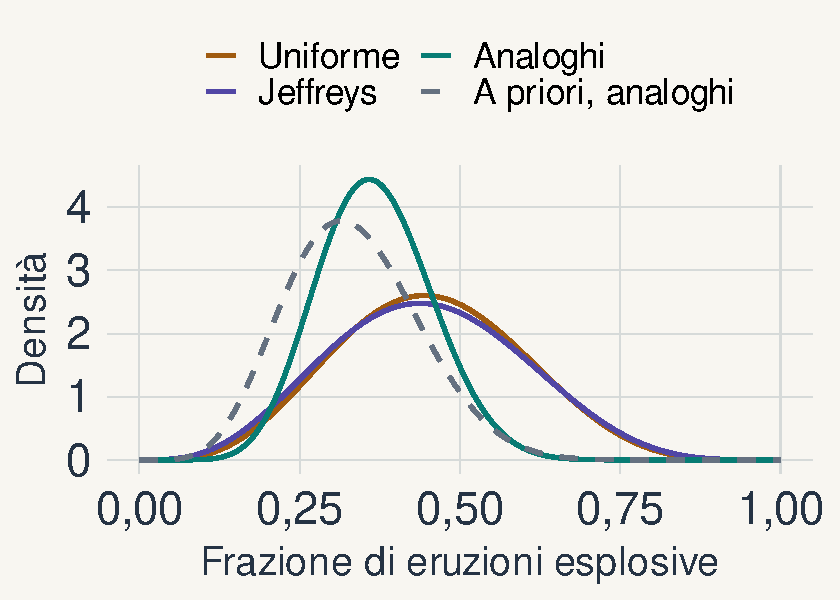
\includegraphics[width=\linewidth,height=6.15cm,keepaspectratio]{Figure/F04.pdf}\par}
\PSmall{Densità a posteriori della frazione esplosiva con tre distribuzioni a priori; tratteggio: beta a priori dei vulcani analoghi.}
}};
\node[anchor=north west,inner sep=0] at([xshift=10.85cm,yshift=-2.12cm]current page.north west){\Colonna{8.16cm}{\PBody{Le distribuzioni a posteriori uniforme e di Jeffreys quasi coincidono: con nove eruzioni la differenza fra le due distribuzioni a priori conta poco. La distribuzione dei vulcani analoghi vale quanto venti eruzioni, più del doppio del registro, e sposta la media a posteriori verso 0,33.}
\PSmall{La forza di una beta a priori è $\alpha+\beta$, il numero di eruzioni a cui equivale.}
}};
\end{tikzpicture}\end{frame}

\begin{frame}[plain]\hypertarget{slide19}{}
\bookmark[level=1,page=19]{E un’eruzione esplosiva?}
\begin{tikzpicture}[remember picture,overlay]
\PilotChrome{E un’eruzione esplosiva?}{SENSIBILITÀ ALLA DISTRIBUZIONE A PRIORI}{19}{La simulazione dalle distribuzioni a posteriori propaga l’incertezza di più parametri.}
\node[anchor=north west,inner sep=0] at([xshift=.96cm,yshift=-2.12cm]current page.north west){\Colonna{9.40cm}{\PLabel{Domanda}
\PBody{Le eruzioni esplosive formano un processo di Poisson con tasso $\lambda p$. Qual è la probabilità di almeno un’eruzione esplosiva nei prossimi cinquant’anni?}
\vspace{.35cm}\PLabel{Interpretazione}
\PBody{Estraendo centomila coppie dalle due distribuzioni a posteriori, la probabilità media vale 0,365. Con le stime puntuali, 2,4 eruzioni per secolo e frazione 4/9, si otterrebbe 0,413.}
}};
\node[anchor=north west,inner sep=0] at([xshift=10.85cm,yshift=-2.12cm]current page.north west){\Colonna{8.16cm}{\begin{tcolorbox}[enhanced,arc=1.7mm,boxrule=.6pt,colback=white,colframe=Classical!60!Navy,colbacktitle=Navy,coltitle=white,fonttitle=\bfseries\small,title={R · calcolo riproducibile},left=1.7mm,right=1.3mm,top=1.1mm,bottom=1.1mm,before skip=1mm,after skip=1.0mm]\lstinputlisting[style=GeoR,language=R]{Codice/capitolo-06.R}\end{tcolorbox}
\PLabel{Risultato in R}
\begin{tcolorbox}[colback=GeoTint,colframe=Rule,boxrule=.5pt,arc=1.4mm,left=2mm,right=1mm,top=1mm,bottom=1mm]{\fontsize{8.6}{11.4}\selectfont\ttfamily \mbox{\ \ \ \ bayes\ con\_stime}\\\mbox{0.3653214\ 0.4133538}}\end{tcolorbox}}};
\end{tikzpicture}\end{frame}

\begin{frame}[plain]\hypertarget{slide20}{}
\bookmark[level=1,page=20]{Quanto conta la distribuzione a priori}
\begin{tikzpicture}[remember picture,overlay]
\PilotChrome{Quanto conta la distribuzione a priori}{SENSIBILITÀ ALLA DISTRIBUZIONE A PRIORI}{20}{Una distribuzione a priori informativa e sbagliata sposta la stima più di quanto i dati possano correggere.}
\node[anchor=north west,inner sep=0] at([xshift=.96cm,yshift=-2.12cm]current page.north west){\Colonna{9.40cm}{{\centering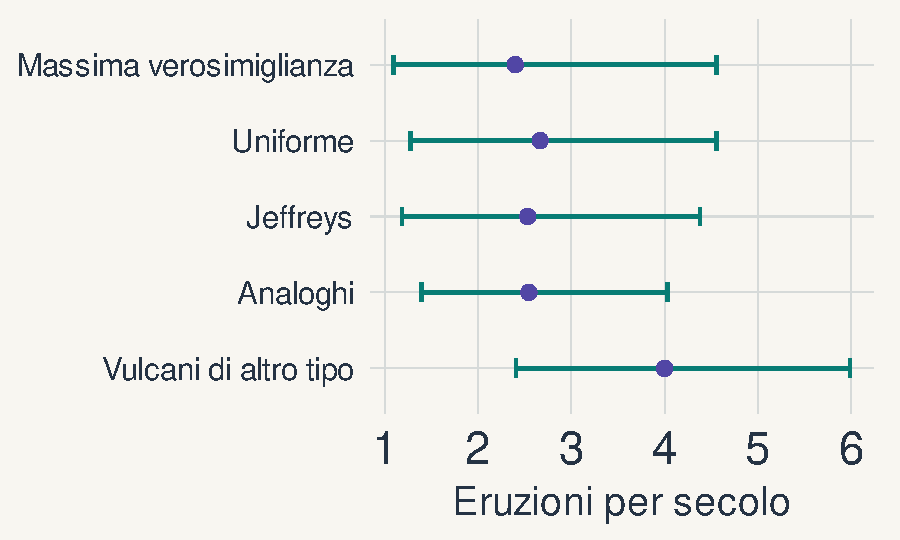
\includegraphics[width=\linewidth,height=6.15cm,keepaspectratio]{Figure/F05.pdf}\par}
\PSmall{Media e intervallo al 95\% del tasso eruttivo con quattro distribuzioni a priori e stima di massima verosimiglianza.}
}};
\node[anchor=north west,inner sep=0] at([xshift=10.85cm,yshift=-2.12cm]current page.north west){\Colonna{8.16cm}{\PBody{Uniforme, Jeffreys e vulcani analoghi danno medie fra 2,53 e 2,67. Una distribuzione a priori tratta da vulcani di altro tipo, gamma con media 10 eruzioni per secolo e forza pari a un secolo, porta la media a 4,00 con intervallo da 2,41 a 5,99. La verosimiglianza normalizzata assegna ai valori oltre 4 una probabilità di 0,07.}
\par\smallskip{\centering\adjustbox{max width=.98\linewidth}{$\displaystyle \frac{a+N}{b+T}=\frac{10+9}{1+3{,}75}=4{,}00$}\par\smallskip}
}};
\end{tikzpicture}\end{frame}

\begin{frame}[plain]\hypertarget{slide21}{}
\bookmark[level=1,page=21]{Che cosa contiene una distribuzione a priori}
\begin{tikzpicture}[remember picture,overlay]
\PilotChrome{Che cosa contiene una distribuzione a priori}{SENSIBILITÀ ALLA DISTRIBUZIONE A PRIORI}{21}{Una distribuzione a priori va dichiarata, giustificata e confrontata con i dati.}
\node[anchor=north west,inner sep=0] at([xshift=.96cm,yshift=-2.12cm]current page.north west){\Colonna{9.40cm}{\PLabel{Dati immaginari}
\PBody{Una gamma con parametri $a$ e $b$ pesa quanto un registro di $b$ secoli con $a$ eruzioni; una beta con parametri $\alpha$ e $\beta$ quanto $\alpha+\beta$ eruzioni. Tradurre la distribuzione a priori in dati equivalenti permette di giudicare se la sua forza è ragionevole: i vulcani analoghi valgono 1,8 secoli e venti eruzioni.}
\par\smallskip{\centering\adjustbox{max width=.98\linewidth}{$\displaystyle w=\frac{b}{b+T}=0{,}325$}\par\smallskip}
}};
\node[anchor=north west,inner sep=0] at([xshift=10.85cm,yshift=-2.12cm]current page.north west){\Colonna{8.16cm}{\PLabel{Controllo predittivo a priori}
\PBody{Prima dell’aggiornamento si chiede quanto sia probabile il dato osservato secondo la distribuzione predittiva a priori. Con i vulcani analoghi un registro con al più nove eruzioni ha probabilità 0,48; con i vulcani di altro tipo 0,0024. Il secondo valore segnala un conflitto fra distribuzione a priori e dati.}
\PSmall{Il controllo segnala un’incoerenza: decidere quale delle due parti sia sbagliata richiede conoscenza geologica.}
}};
\end{tikzpicture}\end{frame}

\begin{frame}[plain]\hypertarget{slide22}{}
\bookmark[level=1,page=22]{Distribuzione a priori in conflitto con i dati}
\begin{tikzpicture}[remember picture,overlay]
\PilotChrome{Distribuzione a priori in conflitto con i dati}{SENSIBILITÀ ALLA DISTRIBUZIONE A PRIORI}{22}{Valutare l’effetto di una distribuzione a priori sbagliata e la capacità del controllo predittivo di rilevarla.}
\node[anchor=north west,inner sep=0] at([xshift=.96cm,yshift=-2.12cm]current page.north west){\Colonna{9.40cm}{{\centering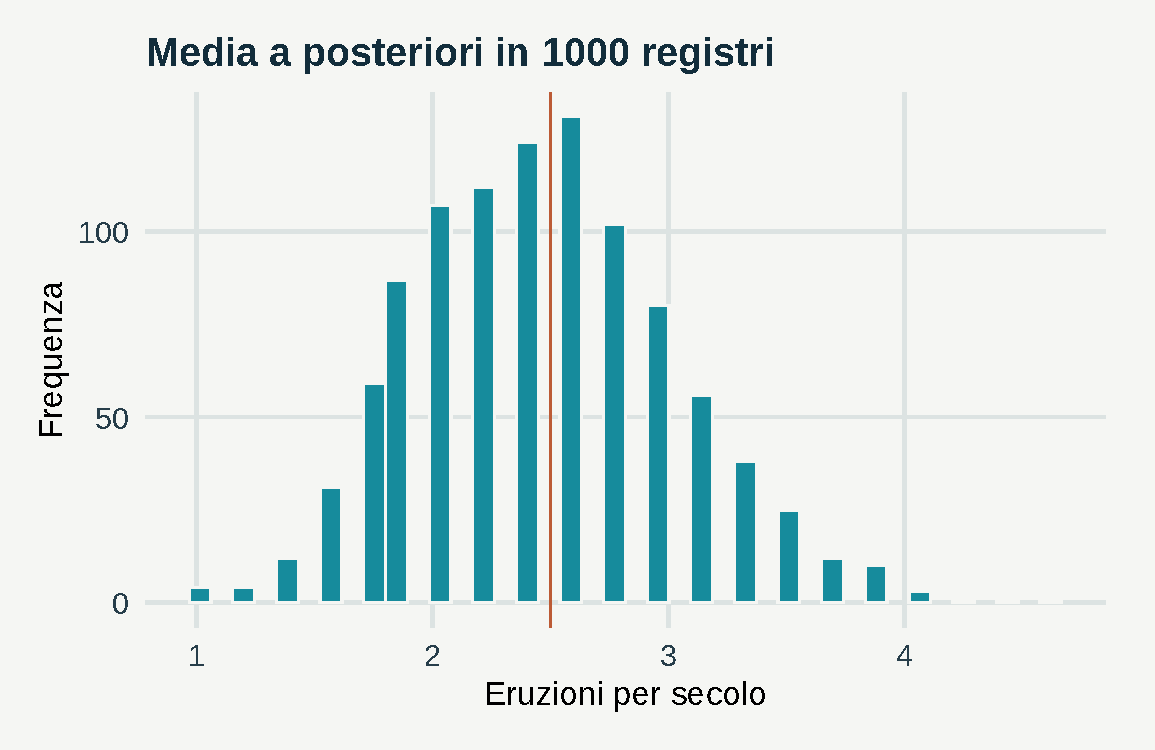
\includegraphics[width=\linewidth,height=6.0cm,keepaspectratio]{Esperimenti/m21-priori-A.pdf}\par}
\PSmall{Media a priori uguale al tasso vero; forza 1,8 secoli; mille registri. Seme: 17.}
}};
\node[anchor=north west,inner sep=0] at([xshift=10.85cm,yshift=-2.12cm]current page.north west){\Colonna{8.16cm}{\PLabel{Scenario A · simulazione}
\PBody{L’esperimento genera mille registri di 3,75 secoli con tasso vero 2,5 e aggiorna una gamma con la media e la forza scelte. Con una distribuzione a priori centrata sul valore vero la media delle medie a posteriori vale 2,48, la copertura 0,974 e il controllo non segnala conflitti.}
\par\smallskip{\centering\adjustbox{max width=.98\linewidth}{$\displaystyle p=2\min\{P(N^\prime\le N),\,P(N^\prime\ge N)\}$}\par\smallskip}
\PSmall{$N^\prime$ segue la distribuzione predittiva a priori, una binomiale negativa.}
}};
\node[anchor=north east,inner sep=0] at([xshift=17.1cm,yshift=-12.04cm]current page.north west){\fontsize{7.7}{9}\selectfont \href{https://marzione00.github.io/Lab_Geo/\#laboratorio/m21-priori}{\color{Classical}\bfseries Apri il laboratorio · m21-priori}};
\end{tikzpicture}\end{frame}

\begin{frame}[plain]\hypertarget{slide23}{}
\bookmark[level=1,page=23]{Confronto | Distribuzione a priori in conflitto}
\begin{tikzpicture}[remember picture,overlay]
\PilotChrome{Confronto | Distribuzione a priori in conflitto}{SENSIBILITÀ ALLA DISTRIBUZIONE A PRIORI}{23}{Una distribuzione a priori sbagliata riduce la copertura; il controllo predittivo la segnala spesso.}
\node[anchor=north west,inner sep=0] at([xshift=.96cm,yshift=-2.12cm]current page.north west){\Colonna{9.40cm}{{\centering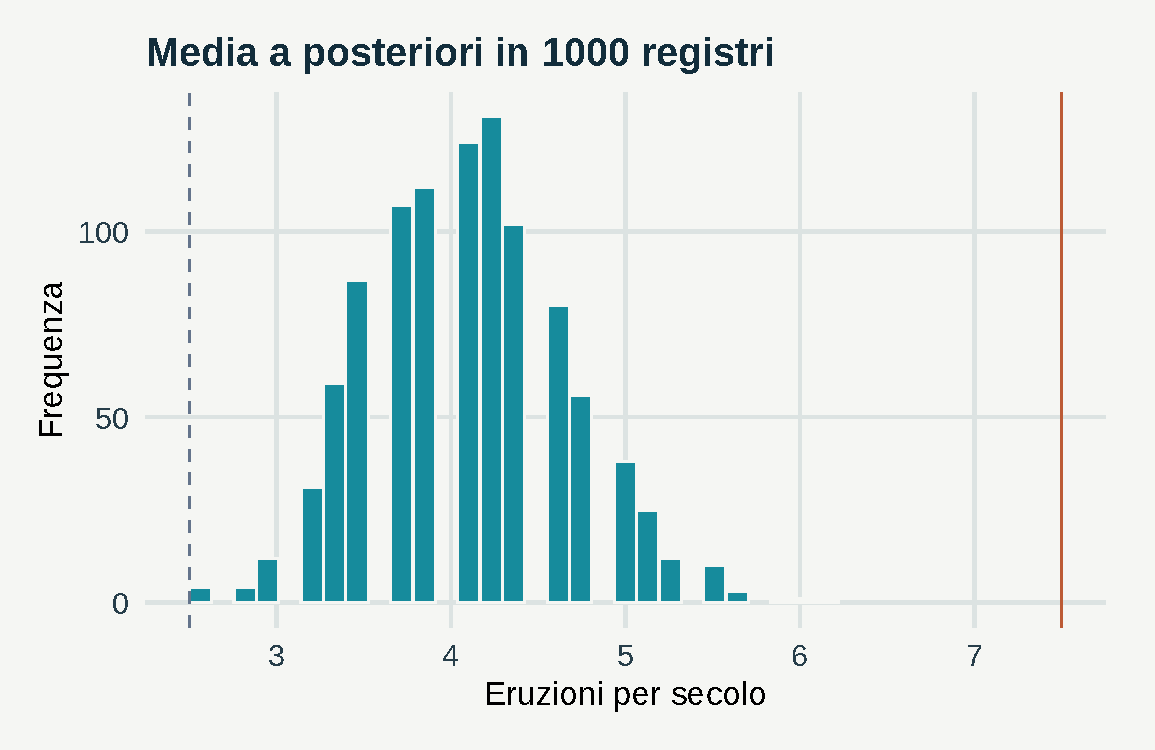
\includegraphics[width=\linewidth,height=5.6cm,keepaspectratio]{Esperimenti/m21-priori-B.pdf}\par}
\PSmall{Media a priori: 1 $\to$ 3 volte il tasso vero. Forza e seme fissi.}
}};
\node[anchor=north west,inner sep=0] at([xshift=10.85cm,yshift=-2.12cm]current page.north west){\Colonna{8.16cm}{\PLabel{Confronto fra gli scenari}
{\fontsize{10.2}{12.8}\selectfont\begin{tabular}{@{}>{\raggedright\arraybackslash}p{0.48\linewidth}@{\hspace{.13cm}}>{\raggedright\arraybackslash}p{0.224\linewidth}@{\hspace{.13cm}}>{\raggedright\arraybackslash}p{0.224\linewidth}@{}}\toprule Grandezza & A & B\\[2.3pt]
\midrule 
Media a priori & 2{,}5 & 7{,}5\\[2.3pt]
Media delle medie a posteriori & 2{,}48 & 4{,}1\\[2.3pt]
Copertura al 95\% & 0{,}974 & 0{,}416\\[2.3pt]
Conflitti segnalati & 0 & 0{,}773\\[2.3pt]
\bottomrule\end{tabular}\par}
\vspace{.25cm}\PBody{Con una media a priori di 7,5 la media a posteriori sale a 4,1 e l’intervallo contiene il valore vero soltanto nel 41,6\% dei registri. Il controllo predittivo segnala il conflitto nel 77,3\% dei casi.}
}};
\node[anchor=north east,inner sep=0] at([xshift=17.1cm,yshift=-12.04cm]current page.north west){\fontsize{7.7}{9}\selectfont \href{https://marzione00.github.io/Lab_Geo/\#laboratorio/m21-priori}{\color{Classical}\bfseries Apri il laboratorio · m21-priori}};
\end{tikzpicture}\end{frame}

\begin{frame}[plain]\hypertarget{slide24}{}
\bookmark[level=0,page=24]{Monte Carlo a catena di Markov}
\bookmark[level=1,page=24]{Le eruzioni sono regolari?}
\begin{tikzpicture}[remember picture,overlay]
\PilotChrome{Le eruzioni sono regolari?}{MONTE CARLO A CATENA DI MARKOV}{24}{Nel processo di Poisson i tempi di riposo sono esponenziali; la Weibull permette tempi più regolari.}
\node[anchor=north west,inner sep=0] at([xshift=.96cm,yshift=-2.12cm]current page.north west){\Colonna{9.40cm}{\PLabel{Domanda}
\PBody{Gli otto tempi di riposo vanno da 20 a 54 anni, e dall’ultima eruzione ne sono passati 37. Il coefficiente di variazione di un processo di Poisson vale 1: quanto vale qui? Che forma stima la Weibull?}
\vspace{.35cm}\PLabel{Interpretazione}
\PBody{Il coefficiente di variazione vale 0,34, e la stima di massima verosimiglianza della forma è 3,96, con scala 44,6 anni. Una forma maggiore di 1 indica un rischio che cresce con il tempo trascorso dall’ultima eruzione.}
}};
\node[anchor=north west,inner sep=0] at([xshift=10.85cm,yshift=-2.12cm]current page.north west){\Colonna{8.16cm}{\begin{tcolorbox}[enhanced,arc=1.7mm,boxrule=.6pt,colback=white,colframe=Classical!60!Navy,colbacktitle=Navy,coltitle=white,fonttitle=\bfseries\small,title={R · calcolo riproducibile},left=1.7mm,right=1.3mm,top=1.1mm,bottom=1.1mm,before skip=1mm,after skip=1.0mm]\lstinputlisting[style=GeoR,language=R]{Codice/capitolo-07.R}\end{tcolorbox}
\PLabel{Risultato in R}
\begin{tcolorbox}[colback=GeoTint,colframe=Rule,boxrule=.5pt,arc=1.4mm,left=2mm,right=1mm,top=1mm,bottom=1mm]{\fontsize{8.6}{11.4}\selectfont\ttfamily \mbox{\ \ \ \ k\ scala}\\\mbox{\ 3.96\ 44.57}\\\mbox{media\ \ \ \ cv}\\\mbox{39.25\ \ 0.34}}\end{tcolorbox}}};
\end{tikzpicture}\end{frame}

\begin{frame}[plain]\hypertarget{slide25}{}
\bookmark[level=1,page=25]{L’algoritmo di Metropolis}
\begin{tikzpicture}[remember picture,overlay]
\PilotChrome{L’algoritmo di Metropolis}{MONTE CARLO A CATENA DI MARKOV}{25}{Metropolis richiede la densità a posteriori soltanto a meno di una costante.}
\node[anchor=north west,inner sep=0] at([xshift=.96cm,yshift=-2.12cm]current page.north west){\Colonna{9.40cm}{{\centering\resizebox{0.94\linewidth}{!}{\begin{tikzpicture}[x=1cm,y=1cm,every node/.append style={anchor=center,inner sep=.3333em}]
\node[pFlow,text width=2.9cm] (a) at(0,2.4){\textbf{1. Stato corrente}\\$\theta^{(t)}$};
\node[pFlow,text width=3.4cm] (b) at(5.6,2.4){\textbf{2. Proposta}\\$\theta^*=\theta^{(t)}+\varepsilon$, $\varepsilon\sim N(0,s^2)$};
\node[pFlow,text width=3.4cm] (c) at(5.6,0){\textbf{3. Rapporto}\\$r=\dfrac{\pi(\theta^*\mid y)}{\pi(\theta^{(t)}\mid y)}$};
\node[pFlow,text width=3.2cm] (d) at(0,0){\textbf{4. Decisione}\\$\theta^{(t+1)}=\theta^*$ con prob. $\min(1,r)$};
\draw[pEdge] (a)--(b);\draw[pEdge] (b)--(c);\draw[pEdge] (c)--(d);\draw[pEdge] (d)--(a);
\node[pNote,text width=7.6cm] at(2.8,-1.65){La costante di normalizzazione si semplifica nel rapporto. Se la proposta è rifiutata, la catena ripete lo stato corrente (Metropolis e colleghi, 1953).};
\end{tikzpicture}
}\par}
\PSmall{Le quattro fasi di un passo della catena.}
}};
\node[anchor=north west,inner sep=0] at([xshift=10.85cm,yshift=-2.12cm]current page.north west){\Colonna{8.16cm}{\PBody{Con due parametri e una distribuzione a priori non coniugata la distribuzione a posteriori non ha una forma nota. Nicholas Metropolis e colleghi proposero nel 1953 una catena di Markov che ha come distribuzione stazionaria quella voluta; W. K. Hastings la generalizzò nel 1970 a proposte asimmetriche.}
\par\smallskip{\centering\adjustbox{max width=.98\linewidth}{$\displaystyle \alpha=\min\Big\{1,\frac{\pi(\theta^*\mid y)}{\pi(\theta^{(t)}\mid y)}\Big\}$}\par\smallskip}
}};
\end{tikzpicture}\end{frame}

\begin{frame}[plain]\hypertarget{slide26}{}
\bookmark[level=1,page=26]{Una catena per la Weibull}
\begin{tikzpicture}[remember picture,overlay]
\PilotChrome{Una catena per la Weibull}{MONTE CARLO A CATENA DI MARKOV}{26}{L’intervallo ancora aperto entra nella verosimiglianza come dato censurato.}
\node[anchor=north west,inner sep=0] at([xshift=.96cm,yshift=-2.12cm]current page.north west){\Colonna{9.40cm}{\PBody{La log-densità a posteriori somma le densità degli otto riposi, la probabilità che il riposo in corso superi 37 anni e due distribuzioni a priori normali sui logaritmi dei parametri. La catena accetta il 41\% delle proposte. Dopo cinquecento iterazioni iniziali la media di $k$ vale 3,15, e $P(k>1)=0{,}994$.}
\par\smallskip{\centering\adjustbox{max width=.98\linewidth}{$\displaystyle \log\pi=\sum_i\log f(r_i)+\log S(37)+\log\pi_0$}\par\smallskip}
}};
\node[anchor=north west,inner sep=0] at([xshift=10.85cm,yshift=-2.12cm]current page.north west){\Colonna{8.16cm}{\begin{tcolorbox}[enhanced,arc=1.7mm,boxrule=.6pt,colback=white,colframe=Classical!60!Navy,colbacktitle=Navy,coltitle=white,fonttitle=\bfseries\small,title={R · calcolo riproducibile},left=1.7mm,right=1.3mm,top=1.1mm,bottom=1.1mm,before skip=1mm,after skip=1.0mm]\lstinputlisting[style=GeoR,language=R]{Codice/capitolo-08.R}\end{tcolorbox}
\PLabel{Risultato in R}
\begin{tcolorbox}[colback=GeoTint,colframe=Rule,boxrule=.5pt,arc=1.4mm,left=2mm,right=1mm,top=1mm,bottom=1mm]{\fontsize{8.6}{11.4}\selectfont\ttfamily \mbox{\ \ acc\ \ \ \ \ k\ \ p\_k1}\\\mbox{0.411\ 3.155\ 0.994}}\end{tcolorbox}}};
\end{tikzpicture}\end{frame}

\begin{frame}[plain]\hypertarget{slide27}{}
\bookmark[level=1,page=27]{La catena e la distribuzione a posteriori della forma}
\begin{tikzpicture}[remember picture,overlay]
\PilotChrome{{\fontsize{15.3}{19}\selectfont La catena e la distribuzione a posteriori della forma}}{MONTE CARLO A CATENA DI MARKOV}{27}{Una traccia stabile e ben mescolata è una condizione necessaria per usare i valori della catena.}
\node[anchor=north west,inner sep=0] at([xshift=.96cm,yshift=-2.12cm]current page.north west){\Colonna{9.40cm}{{\centering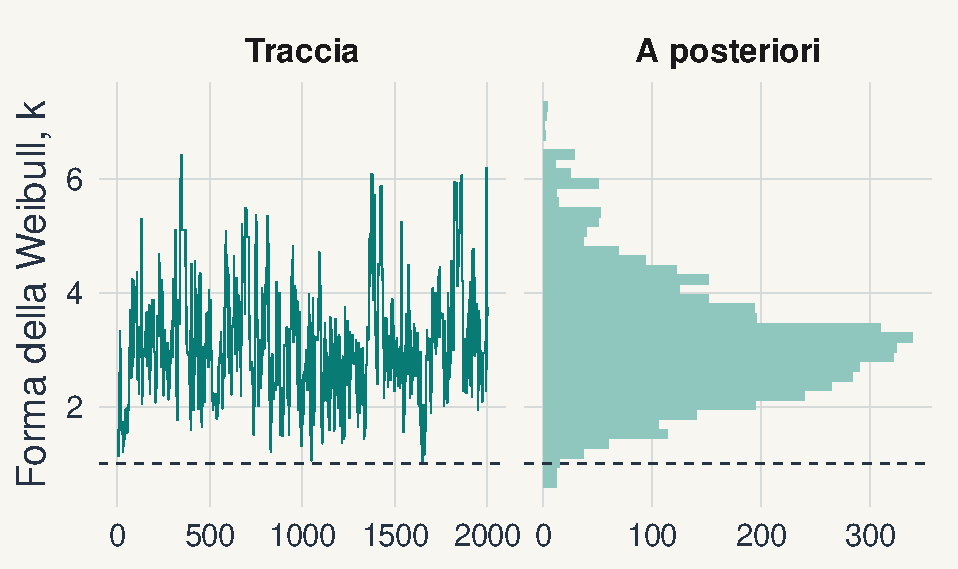
\includegraphics[width=\linewidth,height=6.15cm,keepaspectratio]{Figure/F06.pdf}\par}
\PSmall{Sinistra: prime duemila iterazioni di $k$. Destra: istogramma dei valori dopo le prime cinquecento; tratteggio: $k=1$.}
}};
\node[anchor=north west,inner sep=0] at([xshift=10.85cm,yshift=-2.12cm]current page.north west){\Colonna{8.16cm}{\PBody{La traccia oscilla attorno a 3 senza tendenze dopo le prime iterazioni. L’intervallo al 95\% della forma va da 1,39 a 5,89: i dati escludono il processo di Poisson e lasciano incerta la regolarità. Un’integrazione numerica su griglia dà una media di 3,17.}
\PSmall{Il generatore dei dati usa $k=1{,}8$: otto riposi non bastano a fissare la forma.}
}};
\end{tikzpicture}\end{frame}

\begin{frame}[plain]\hypertarget{slide28}{}
\bookmark[level=1,page=28]{Diagnostica e uso della catena}
\begin{tikzpicture}[remember picture,overlay]
\PilotChrome{Diagnostica e uso della catena}{MONTE CARLO A CATENA DI MARKOV}{28}{Valori autocorrelati contengono meno informazione di altrettante estrazioni indipendenti.}
\node[anchor=north west,inner sep=0] at([xshift=.96cm,yshift=-2.12cm]current page.north west){\Colonna{9.40cm}{\PLabel{Controllare la catena}
\PBody{I valori iniziali dipendono dal punto di partenza e si scartano. I valori successivi sono autocorrelati: la dimensione campionaria efficace dei 4500 valori di $k$ è circa 170. A. Gelman e D. B. Rubin proposero nel 1992 di lanciare più catene da punti di partenza dispersi e di confrontare la variabilità fra catene ed entro catene.}
\par\smallskip{\centering\adjustbox{max width=.98\linewidth}{$\displaystyle n_{\mathrm{eff}}=\frac{n}{1+2\sum_{l}\rho_l}$}\par\smallskip}
}};
\node[anchor=north west,inner sep=0] at([xshift=10.85cm,yshift=-2.12cm]current page.north west){\Colonna{8.16cm}{\PLabel{Una probabilità condizionata}
\PBody{Ogni valore della catena dà una probabilità di eruzione nei prossimi cinquant’anni, dati i 37 anni già trascorsi; la media vale 0,97. Il processo di Poisson, privo di memoria, dà 0,70. Con la forma del generatore, 1,8, la probabilità vera è 0,91.}
\PSmall{$P=1-\exp\{(37/\eta)^k-(87/\eta)^k\}$, mediata sui valori della catena.}
}};
\end{tikzpicture}\end{frame}

\begin{frame}[plain]\hypertarget{slide29}{}
\bookmark[level=1,page=29]{Passo della proposta e mescolamento della catena}
\begin{tikzpicture}[remember picture,overlay]
\PilotChrome{Passo della proposta e mescolamento della catena}{MONTE CARLO A CATENA DI MARKOV}{29}{Valutare come il passo della proposta cambia accettazione, autocorrelazione e precisione.}
\node[anchor=north west,inner sep=0] at([xshift=.96cm,yshift=-2.12cm]current page.north west){\Colonna{9.40cm}{{\centering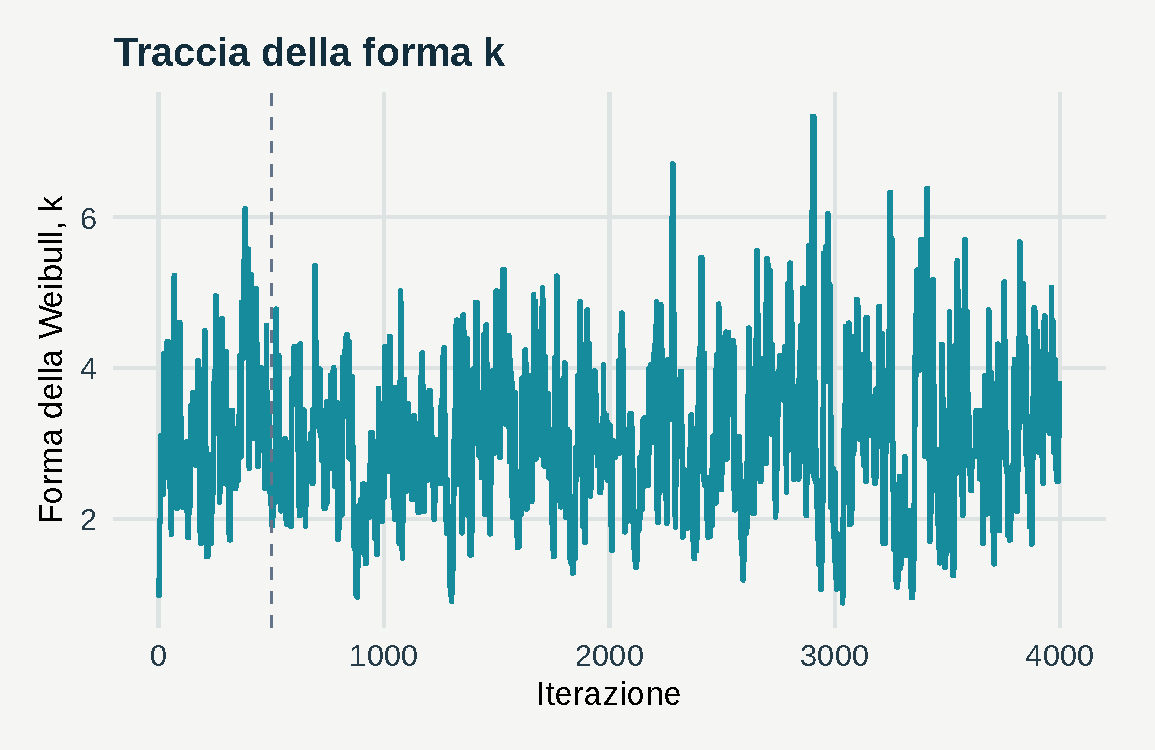
\includegraphics[width=\linewidth,height=6.0cm,keepaspectratio]{Esperimenti/m21-metropolis-A.pdf}\par}
\PSmall{Passo 0,25 sulla scala logaritmica; quattromila iterazioni. Seme: 17.}
}};
\node[anchor=north west,inner sep=0] at([xshift=10.85cm,yshift=-2.12cm]current page.north west){\Colonna{8.16cm}{\PLabel{Scenario A · simulazione}
\PBody{L’esperimento esegue l’algoritmo di Metropolis sui tempi di riposo del caso con il passo scelto. Con passo 0,25 la catena accetta il 43\% delle proposte, la media di $k$ vale 3,10 e la dimensione campionaria efficace 212.}
\par\smallskip{\centering\adjustbox{max width=.98\linewidth}{$\displaystyle \theta^*=\theta^{(t)}+\varepsilon,\quad\varepsilon\sim N(0,s^2I)$}\par\smallskip}
\PSmall{Il valore di riferimento, 3,17, viene dall’integrazione su griglia.}
}};
\node[anchor=north east,inner sep=0] at([xshift=17.1cm,yshift=-12.04cm]current page.north west){\fontsize{7.7}{9}\selectfont \href{https://marzione00.github.io/Lab_Geo/\#laboratorio/m21-metropolis}{\color{Classical}\bfseries Apri il laboratorio · m21-metropolis}};
\end{tikzpicture}\end{frame}

\begin{frame}[plain]\hypertarget{slide30}{}
\bookmark[level=1,page=30]{Confronto | Passo della proposta}
\begin{tikzpicture}[remember picture,overlay]
\PilotChrome{Confronto | Passo della proposta}{MONTE CARLO A CATENA DI MARKOV}{30}{Un passo troppo piccolo accetta quasi tutto ed esplora poco.}
\node[anchor=north west,inner sep=0] at([xshift=.96cm,yshift=-2.12cm]current page.north west){\Colonna{9.40cm}{{\centering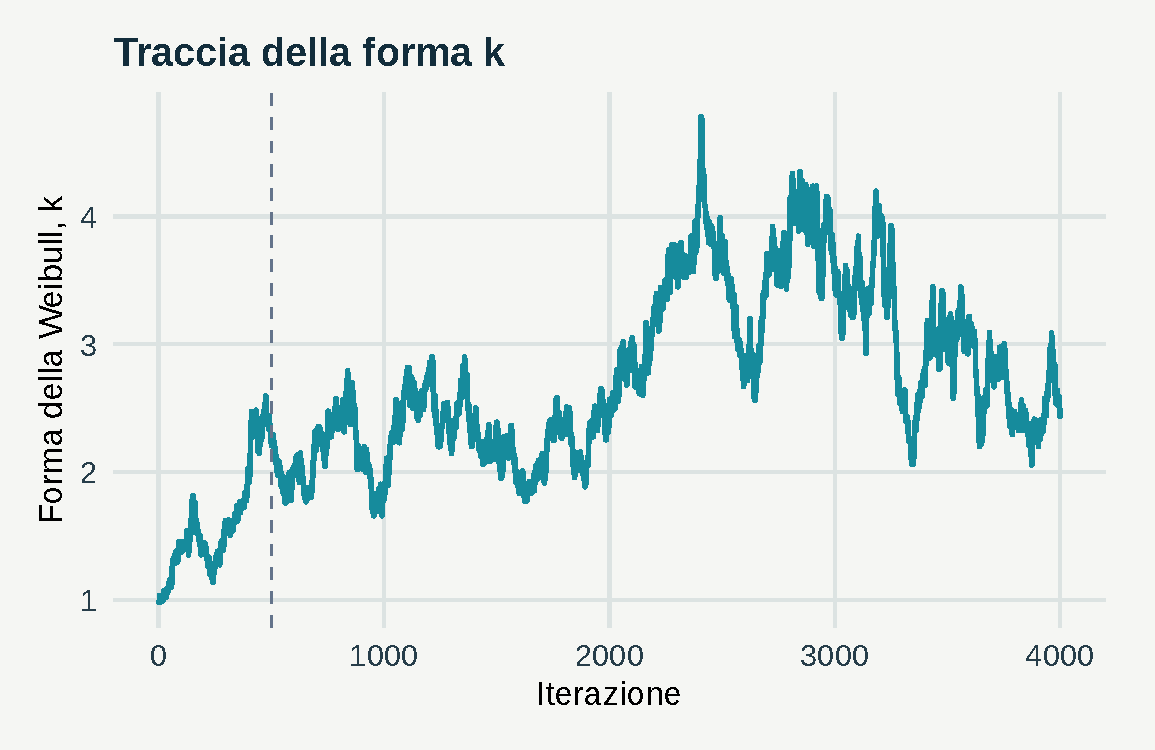
\includegraphics[width=\linewidth,height=5.6cm,keepaspectratio]{Esperimenti/m21-metropolis-B.pdf}\par}
\PSmall{Passo della proposta: 0,25 $\to$ 0,02. Il seme è fisso.}
}};
\node[anchor=north west,inner sep=0] at([xshift=10.85cm,yshift=-2.12cm]current page.north west){\Colonna{8.16cm}{\PLabel{Confronto fra gli scenari}
{\fontsize{10.2}{12.8}\selectfont\begin{tabular}{@{}>{\raggedright\arraybackslash}p{0.48\linewidth}@{\hspace{.13cm}}>{\raggedright\arraybackslash}p{0.224\linewidth}@{\hspace{.13cm}}>{\raggedright\arraybackslash}p{0.224\linewidth}@{}}\toprule Grandezza & A & B\\[2.3pt]
\midrule 
Tasso di accettazione & 0{,}433 & 0{,}946\\[2.3pt]
Media a posteriori di k & 3{,}1 & 2{,}78\\[2.3pt]
Dimensione campionaria efficace & 212 & 11{,}9\\[2.3pt]
Riferimento su griglia & 3{,}17 & 3{,}17\\[2.3pt]
\bottomrule\end{tabular}\par}
\vspace{.25cm}\PBody{Con passo 0,02 la catena accetta il 94,6\% delle proposte ma si sposta di poco a ogni passo: la dimensione campionaria efficace scende a 11,9 e la media di $k$, 2,78, risente ancora del punto di partenza.}
}};
\node[anchor=north east,inner sep=0] at([xshift=17.1cm,yshift=-12.04cm]current page.north west){\fontsize{7.7}{9}\selectfont \href{https://marzione00.github.io/Lab_Geo/\#laboratorio/m21-metropolis}{\color{Classical}\bfseries Apri il laboratorio · m21-metropolis}};
\end{tikzpicture}\end{frame}

\begin{frame}[plain]\hypertarget{slide31}{}
\bookmark[level=0,page=31]{Sintesi}
\bookmark[level=1,page=31]{Dal risultato alla relazione}
\begin{tikzpicture}[remember picture,overlay]
\PilotChrome{Dal risultato alla relazione}{SINTESI}{31}{Riporta distribuzione a priori e sua origine, distribuzione a posteriori, controlli e probabilità predittive.}
\node[anchor=north west,inner sep=0] at([xshift=.96cm,yshift=-2.12cm]current page.north west){\Colonna{9.40cm}{\PLabel{Domanda di partenza}
\PBody{Quanto è probabile un’eruzione nei prossimi cinquant’anni?}
\PLabel{Risultato da discutere}
\PBody{Il tasso eruttivo ha media a posteriori di 2,55 eruzioni per secolo, con intervallo di credibilità al 95\% da 1,4 a 4,0; la probabilità di almeno un’eruzione nei prossimi cinquant’anni è 0,70 con il processo di Poisson, e quella di un’eruzione esplosiva 0,37. I tempi di riposo sono più regolari di un processo di Poisson, e con 37 anni già trascorsi il modello di Weibull porta la probabilità a 0,97.}
}};
\node[anchor=north west,inner sep=0] at([xshift=10.85cm,yshift=-2.12cm]current page.north west){\Colonna{8.16cm}{\PLabel{Limiti della conclusione}
\PBody{I dati sono sintetici e il registro storico è considerato completo. La forma della Weibull è incerta, da 1,4 a 5,9, e la probabilità condizionata dipende da essa; i vulcani analoghi sono scambiabili con il caso per ipotesi.}
\vspace{.4cm}\href{https://marzione00.github.io/Lab_Geo/\#modulo-M21}{\color{Classical}\bfseries Torna agli esperimenti di Credentia}
}};
\end{tikzpicture}\end{frame}

\begin{frame}[plain]\hypertarget{slide32}{}
\bookmark[level=0,page=32]{Riferimenti}
\bookmark[level=1,page=32]{Fonti, dati e codice per riprodurre le figure}
\begin{tikzpicture}[remember picture,overlay]
\PilotChrome{Fonti, dati e codice per riprodurre le figure}{RIFERIMENTI}{32}{I risultati numerici si riferiscono ai dati e alle ipotesi dichiarate nel caso.}
\node[anchor=north west,inner sep=0] at([xshift=.96cm,yshift=-2.12cm]current page.north west){\Colonna{9.40cm}{\PLabel{Fonti}
{\fontsize{9.4}{12.2}\selectfont T. Bayes, Philosophical Transactions of the Royal Society 53, 370–418, 1763.\par F. Garwood, Biometrika 28(3–4), 437–442, 1936.\par H. Jeffreys, Proceedings of the Royal Society A 186, 453–461, 1946.\par N. Metropolis, A. W. Rosenbluth, M. N. Rosenbluth, A. H. Teller e E. Teller, Journal of Chemical Physics 21(6), 1087–1092, 1953.\par W. K. Hastings, Biometrika 57(1), 97–109, 1970.\par A. Gelman e D. B. Rubin, Statistical Science 7(4), 457–472, 1992.\par C. G. Newhall e R. P. Hoblitt, Bulletin of Volcanology 64, 3–20, 2002.\par W. Marzocchi, L. Sandri e J. Selva, Bulletin of Volcanology 70(5), 623–632, 2008.\par M. S. Bebbington, Statistics in Volcanology 1, 1–24, 2013.\par}
}};
\node[anchor=north west,inner sep=0] at([xshift=10.85cm,yshift=-2.12cm]current page.north west){\Colonna{8.16cm}{\PLabel{Dati e codice}
\PBody{Dati sintetici del corso (eruzioni\_v1.csv, analoghi\_v1.csv), generati da R/genera\_dati.R. Codice contiene i frammenti delle pagine; R/M21\_figure.R ricostruisce figure e valori; Esperimenti contiene i programmi dei due scenari e Diagrammi i disegni TikZ.}
\vspace{.3cm}\href{https://marzione00.github.io/Lab_Geo/\#lezione-M21}{\color{Classical}\bfseries Apri le tappe di Credentia su GeoStat Lab}
}};
\end{tikzpicture}\end{frame}
\end{document}
